\documentclass[article, 11pt]{IEEEtran}   %Document is an article, 11 pt font, and follows IEEE format

%Paquetes
\usepackage{hyperref}         %hiperlinks
\usepackage{graphicx}         %imágenes
\usepackage{float}            %posicionar imágenes
\usepackage{gensymb}          %símbolos
\usepackage{amsmath,amssymb}   %fórmulas matemáticas
\usepackage{booktabs}         %tablas
\usepackage{tikz}             %esquemas
\usetikzlibrary{arrows.meta,positioning}
\usepackage[utf8]{inputenc}
\usepackage[T1]{fontenc}
\usepackage[spanish,es-noshorthands]{babel}   %caracteres en español
\AtBeginDocument{\renewcommand{\%}{\char37\relax}}   % evita conflicto de babel con \,\%
\hypersetup{hidelinks}
\graphicspath{{imgs/}}

\begin{document}

\title{Modelado y Simulaci\'on de un Cohete en el Plano de Cabeceo:\\ Estabilidad, Acoplamiento y Selecci\'on de Ganancias}

\author{\IEEEauthorblockN{Jos\'e Barreno\\Luis Guzm\'an\\Byron Garc\'ia\\Jos\'e Rivera}
\IEEEauthorblockA{\\Universidad Galileo, Teor\'ia de Sistemas II\\Guatemala, Guatemala}}

\maketitle

%====================================================================
\begin{abstract}
Un cohete no solo debe acelerar: tambi\'en debe tener una direccion, este trabajo estudia el modelo lineal de un cohete en el plano de cabeceo, con dos entradas (comando de aceleraci\'on axial y de \'angulo de cabeceo), dos salidas (aceler\'ometro e IMU) y dos ganancias, $K_1$ y $K_2$, cuyo efecto se estara analizando. Se obtiene la matriz de transferencia, se estudia la estabilidad, la respuesta en el tiempo y en frecuencia, el acoplamiento entre canales, la observabilidad y la controlabilidad, y se elige un rango de ganancias y un periodo de muestreo, el cohete es inestable por naturaleza (la aerodin\'amica lo vuelca) y lo estabiliza la tobera: basta $K_2\gtrsim0{,}09$, con las ganancias de partida $(1;0{,}5)$ el acoplamiento por gravedad es de 177~\% ($u_2\to a$) y 21~\% ($u_1\to\theta$), el rango recomendado, $K_1\in[4;6{,}5]$ y $K_2\in[1{,}1;1{,}45]$, reduce el sobrepaso de 16,4~\% a 0,8~\% y el tiempo de asentamiento de 3,6 s a 1,6 s, y reparte el acoplamiento (31~\% y 28~\%). Con esas ganancias, un periodo de muestreo de 0,05 s es suficiente: el periodo m\'aximo estable (0,114 s) es $2{,}3$ veces mayor, incluso con un retardo de c\'omputo. Se plantea adem\'as c\'omo cambiar\'ia el modelo con masa variable y con un canal de gui\~nada, dado que son modelos que se acercan mas a la realidad.
\end{abstract}

%====================================================================
\section{Introducci\'on}
Para que una misi\'on espacial tenga \'exito no basta con que el cohete acelere correctamente, tambi\'en debe apuntar correctamente, un error de pocos grados en la actitud durante el ascenso se convierte en desviaciones de kil\'ometros al insertar la carga en \'orbita, y en cargas aerodin\'amicas que pueden destruir la estructura, por eso un cohete no es un sistema de una entrada y una salida, es un sistema \emph{multivariable} (MIMO)~\cite{skogestad}, con un canal de empuje que gobierna la aceleraci\'on y un canal de direcci\'on que gobierna el \'angulo de cabeceo.

Los dos canales no son independientes, la tobera que corrige la direcci\'on tambi\'en desv\'ia el empuje y al inclinar el cohete, la gravedad le resta aceleraci\'on axial, y un aumento del empuje, ante una peque\~na desalineaci\'on del motor, perturba la actitud, esta interacci\'on cruzada (acoplamiento) es el fen\'omeno central del trabajo, una forma de controlar la direcci\'on es orientar la tobera, existen otros como, aletas, cohetes vernier, paletas de chorro ~\cite{nasa}, aqu\'i se modela el empuje orientable con las hip\'otesis cl\'asicas de un modelo de cabeceo linealizado~\cite{wie,greensite}.

El trabajo busca responder seis preguntas, que ordenan el resto del reporte:
\begin{enumerate}
  \item ¿Qu\'e hace cada parte del modelo y c\'omo se conectan los dos canales?
  \item ¿Es estable el cohete y para qu\'e ganancias $K_1,K_2$?
  \item ¿Cu\'anto, y a qu\'e frecuencias, se acoplan los canales? ¿Cu\'ando es razonable tratarlos como independientes?
  \item ¿Se puede \emph{ver} y \emph{mover} todo el estado con los sensores y actuadores disponibles?
  \item ¿Qu\'e ganancias y qu\'e periodo de muestreo conviene elegir?
  \item ¿Qu\'e cambiar\'ia si la masa disminuyera durante el vuelo o si se incluyera la gui\~nada?
\end{enumerate}
La hip\'otesis de trabajo es que la gravedad domina el acoplamiento, que $K_2$ (tobera) gobierna la estabilidad y la actitud mientras que $K_1$ (motor) gobierna la aceleraci\'on, y que existe un rango de $(K_1,K_2)$ con respuesta estable, r\'apida y con tobera y acoplamiento aceptables, la metodolog\'ia combina el modelo en espacio de estados, la matriz de transferencia, simulaci\'on en el tiempo, an\'alisis en frecuencia y un modelo muestreado, se espera encontrar una zona de ganancias bien definida y un periodo de muestreo con margen suficiente.

%====================================================================
\section{Metodolog\'ia}

\subsection*{Modelo}
Se modela solo el plano de cabeceo durante la fase atmosf\'erica del ascenso, con las hip\'otesis habituales de un modelo linealizado, movimiento en el plano, \'angulos peque\~nos ($\sin\theta\approx\theta$), masa, inercia y presi\'on din\'amica constantes en la ventana de an\'alisis, motor con retardo de primer orden $\tau_m$ (una subida exponencial, sin tiempo muerto) y servo de la tobera con $\tau_s\ll\tau_m$, y fuselaje r\'igido sin oleaje del propelente, el estado es $x=[a,\theta,\omega,\delta]^T$, aceleraci\'on axial, \'angulo de cabeceo, velocidad de cabeceo y deflexi\'on de la tobera, las entradas son $u_1$ (comando de aceleraci\'on axial, en \%) y $u_2$ (comando de \'angulo, en rad); las salidas medidas, $y=[a,\theta]^T$, con las ganancias ya incorporadas en el modelo,
\begin{align}
\dot a &= -\tfrac{1+K_1k_a}{\tau_m}\,a-c_\theta\,\theta+\tfrac{K_1k_a}{\tau_m}\,u_1,\label{eq:a}\\
\dot\theta &= \omega,\label{eq:th}\\
\dot\omega &= \mu\,\theta-a_d\,\omega+k_\delta\,\delta+k_\varepsilon\,a,\label{eq:om}\\
\dot\delta &= -\tfrac{1}{\tau_s}\,\delta-\tfrac{K_2}{\tau_s}\,\theta-\tfrac{\lambda K_2}{\tau_s}\,\omega+\tfrac{K_2}{\tau_s}\,u_2.\label{eq:de}
\end{align}
Detr\'as hay un controlador, las leyes $v_1=K_1(u_1-a)$ y $v_2=K_2(u_2-\theta-\lambda\omega)$, donde $\lambda\omega$ aporta amortiguamiento, por eso $K_1$ y $K_2$ aparecen \emph{dentro} de las matrices del modelo, cambiar una ganancia cambia la din\'amica del cohete en lazo cerrado, los valores nominales se resumen en la tabla~\ref{tab:param}; las ganancias de partida son $K_1=1$, $K_2=0{,}5$ y el periodo de muestreo $T=0{,}05$ s.

\begin{table}[!t]
\centering\small
\caption{Par\'ametros nominales del modelo.}\label{tab:param}
\begin{tabular}{p{0.9cm}p{2.4cm}p{3.6cm}}
\toprule
S\'imbolo & Valor & Papel f\'isico\\
\midrule
$k_a$ & 0,0655 (m/s$^2$)/\% & ganancia del actuador de empuje\\
$1/\tau_m$ & 1,0672 s$^{-1}$ & rapidez del motor ($\tau_m\approx0{,}94$ s)\\
$c_\theta$ & 9,81 (m/s$^2$)/rad & gravedad, p\'erdida de aceleraci\'on al inclinarse\\
$\mu$ & 1,20 s$^{-2}$ & rigidez aerodin\'amica (desestabiliza)\\
$a_d$ & 0,35 s$^{-1}$ & amortiguamiento aerodin\'amico\\
$k_\delta$ & 8,50 s$^{-2}$/rad & efectividad de la tobera\\
$k_\varepsilon$ & 0,12 rad/m & desalineaci\'on del empuje\\
$1/\tau_s$ & 20 s$^{-1}$ & rapidez del servo ($\tau_s=0{,}05$ s)\\
$\lambda$ & 0,60 s & peso de $\omega$ en la IMU\\
\bottomrule
\end{tabular}
\end{table}

\subsection*{Herramientas y procedimiento}
Todo el c\'alculo se realiz\'o en Python (NumPy, SciPy, SymPy y Matplotlib), con una funci\'on para cada tipo de an\'alisis, la matriz de transferencia $G(p)=C(pI-A)^{-1}B$ se obtiene de forma simb\'olica y num\'erica ($p$ es la variable de Laplace), la estabilidad se estudia con el criterio de Routh--Hurwitz~\cite{ogata} y se verific\'a contra el c\'alculo directo de los autovalores en 4941 pares $(K_1,K_2)$, sin ning\'un desacuerdo, las respuestas en el tiempo se simulan con SciPy, la respuesta en frecuencia se obtiene evaluando $G(j\omega)$ entre $10^{-3}$ y $10^{3}$ rad/s.

Cuando hace falta comparar efectos de unidades distintas (aceleraci\'on en m/s$^2$ y \'angulo en rad) se aplican escalones de $u_1=10$~\% de empuje y $u_2=5^\circ$, estas magnitudes son una elecci\'on del equipo, se escogieron para mantener el \'angulo de cabeceo y la deflexi\'on de tobera en pocos grados, donde el modelo lineal es v\'alido, los dos porcentajes de acoplamiento dependen de la relaci\'on $u_2/u_1$, por lo que se reportan para este par de escalones.

El muestreo se modela separando el cohete (planta, continua) del controlador (la computadora), solo la realimentaci\'on se muestrea, cada $T$ segundos (el periodo de muestreo, de 0,05 s como valor de partida) la computadora lee los sensores y calcula una orden, y la mantiene constante hasta la siguiente muestra (retenedor de orden cero, como un convertidor D/A real), si se discretizara la matriz $A$ ya cerrada, el controlador y el cohete quedar\'ian mezclados y el resultado ser\'ia enga\~noso, se estudian dos casos, computadora instant\'anea y con retardo de una muestra, la estabilidad discreta se juzga con el radio espectral (mayor m\'odulo de los autovalores), menor que 1, estable~\cite{franklin}.

%====================================================================
\section{Resultados y Discusi\'on}

\subsection*{Estructura y din\'amica del cohete}
\textbf{Los bloques.} El sistema tiene cinco partes, y la se\~nal las recorre en este orden, los \emph{sensores}, un aceler\'ometro y una IMU, miden $a$ y $\theta$ (y $\omega$, que la IMU tambi\'en entrega) como se\~nales anal\'ogicas continuas, un convertidor \emph{A/D} (anal\'ogico--digital), a la entrada de la computadora, toma una lectura de esas se\~nales cada $T$ segundos y la convierte en n\'umeros, la \emph{computadora de a bordo} trabaja solo con esos n\'umeros, recibe los comandos $u_1$ y $u_2$ (datos de seguimiento de la trayectoria), los compara con lo medido y aplica las ganancias $K_1$ y $K_2$ para calcular las \'ordenes $v_1$ y $v_2$, un convertidor \emph{D/A} (digital--anal\'ogico), a la salida de la computadora, transforma esas \'ordenes en se\~nales anal\'ogicas y mantiene cada una constante hasta la siguiente muestra, los \emph{amplificadores de potencia} elevan esas se\~nales al nivel que necesitan el motor y el servo de la tobera, finalmente est\'a la \emph{din\'amica del cohete}, continua, cuyas salidas vuelven a los sensores, el muestreo ocurre entonces en las dos interfaces de la computadora, el A/D de entrada y el D/A de salida, entre ellas todo es discreto, y el resto del lazo (amplificadores, motor, servo, cohete y sensores) es continuo, el modelo supone conversiones ideales, ignora la cuantizaci\'on y el tiempo de conversi\'on, y conserva solo el efecto del periodo $T$ y del mantenimiento de la orden.

\textbf{La cadena causa--efecto.} Las ecuaciones~(\ref{eq:a})--(\ref{eq:de}) se leen como frases (figura~\ref{fig:cadena}), al mover la tobera ($\delta$) se produce un momento que hace girar al cohete ($\omega$) y, integrando, inclinarlo ($\theta$), es el camino principal de actitud, $u_2\to\delta\to\omega\to\theta$, la inclinaci\'on tiene dos consecuencias, la primera es el \emph{acoplamiento por gravedad}, parte del peso queda alineado con el eje y le quita aceleraci\'on ($-c_\theta\theta$ en la ec.~\ref{eq:a}), de modo que \emph{inclinar el cohete reduce su aceleraci\'on axial}, la segunda es el vuelco aerodin\'amico $\mu\theta$ en la ec.~(\ref{eq:om}), con $\mu=1{,}2>0$, cuanto m\'as inclinado, m\'as lo empuja el aire para inclinarlo m\'as, como una flecha con las plumas al rev\'es, por eso el cohete es \emph{inestable por naturaleza}, en sentido inverso, el empuje ($u_1\to a$) alimenta $\dot\omega$ mediante $k_\varepsilon$, acelerar inclina un poco al cohete (acoplamiento $u_1\to\theta$), El resto del an\'alisis examina esta cadena desde distintos \'angulos.

\begin{figure}[!t]
\centering
\resizebox{\columnwidth}{!}{%
\begin{tikzpicture}[>=Stealth,node distance=1.35cm,
  box/.style={draw,rounded corners,minimum width=1.1cm,minimum height=0.75cm,fill=blue!5},
  inp/.style={draw,rounded corners,minimum width=0.9cm,minimum height=0.65cm,fill=orange!15}]
  \node[inp] (u2) {$u_2$};
  \node[box,right=of u2] (d) {$\delta$};
  \node[box,right=of d] (w) {$\omega$};
  \node[box,right=of w] (t) {$\theta$};
  \node[box,right=of t] (a) {$a$};
  \node[inp,below=1.2cm of a] (u1) {$u_1$};
  \draw[->] (u2)--(d) node[midway,above,font=\scriptsize]{servo};
  \draw[->] (d)--(w) node[midway,above,font=\scriptsize]{$k_\delta$};
  \draw[->] (w)--(t) node[midway,above,font=\scriptsize]{$\int$};
  \draw[->] (t)--(a) node[midway,above,font=\scriptsize]{$-c_\theta$};
  \draw[->] (u1)--(a);
  \draw[->] (a) to[bend left=35] node[midway,above,font=\scriptsize]{$k_\varepsilon$} (w);
  \draw[->] (t) to[bend right=55] node[midway,above,font=\scriptsize]{$\mu$ (inestable)} (w);
\end{tikzpicture}}
\caption{Cadena causa--efecto del cohete, las flechas $-c_\theta$ y $k_\varepsilon$ son los dos acoplamientos entre canales.}\label{fig:cadena}
\end{figure}

\textbf{El papel de $K_1$ y $K_2$.} $K_1$ pertenece al canal del motor, aparece en el coeficiente $(1+K_1k_a)/\tau_m$ de la ec.~(\ref{eq:a}), al subir $K_1$ de 1 a 20, ese coeficiente pasa de 1,14 a 2,46 s$^{-1}$, el tiempo caracter\'istico del motor baja de 0,88 s a 0,41 s y la aceleraci\'on final por unidad de comando sube de 0,06 a 0,57 (sin gravedad), es decir, el canal responde m\'as r\'apido y con menos error, sigue la orden m\'as de cerca, $K_2$ pertenece al servo, es la fuerza con que la tobera corrige el \'angulo y la velocidad de giro, y es lo \'unico que combate la inestabilidad aerodin\'amica.

\textbf{El diagrama de simulaci\'on.} Cada entrada distinta de cero en $A$ o $B$ es una flecha del diagrama de la figura~\ref{fig:diagrama}, cuyas ganancias $g_1,\dots,g_{10}$ se resumen en la tabla~\ref{tab:g}, se verific\'o trayectoria por trayectoria que el diagrama coincide con las ecuaciones~(\ref{eq:a})--(\ref{eq:de}), Si $K_2=0$ desaparecen $g_8$ (el orden y la correcci\'on de \'angulo que recibe el servo) y $g_9$ (el amortiguamiento artificial por velocidad de giro), el servo no recibe ninguna orden y la tobera queda quieta, si no hubiera acoplamiento cruzado ($c_\theta=0$ y $k_\varepsilon=0$) desaparecer\'ian $g_2$ (la gravedad, flecha $\theta\to a$) y $g_4$ (la desalineaci\'on del empuje, flecha $a\to\omega$) y los dos canales ser\'ian independientes.

\begin{figure}[!t]
\centering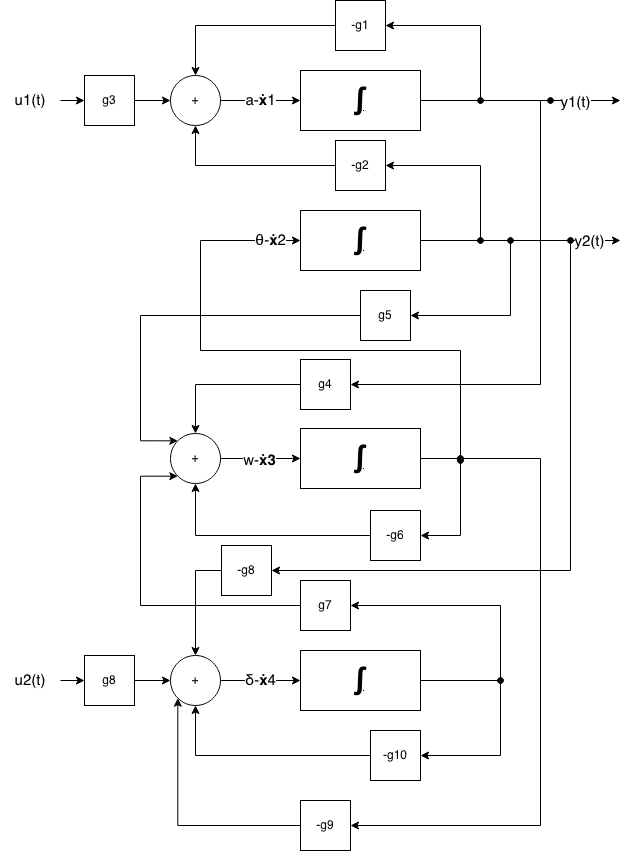
\includegraphics[width=0.78\columnwidth]{TSII - Simulation Diagram.drawio.png}
\caption{Diagrama de simulaci\'on del cohete (cuatro integradores, uno por estado).}\label{fig:diagrama}
\end{figure}

\begin{table}[!t]
\centering\footnotesize\setlength{\tabcolsep}{3pt}
\caption{Ganancias del diagrama de simulaci\'on (valores con $K_1=1$, $K_2=0{,}5$).}\label{tab:g}
\begin{tabular}{llrp{3.3cm}}
\toprule
 & Expresi\'on & Valor & Camino que representa\\
\midrule
$g_1$ & $(1+K_1k_a)/\tau_m$ & 1,137 & $a\to\dot a$ ($-$), retardo del motor y realimentaci\'on del aceler\'ometro\\
$g_2$ & $c_\theta$ & 9,81 & $\theta\to\dot a$ ($-$), p\'erdida de aceleraci\'on por gravedad\\
$g_3$ & $K_1k_a/\tau_m$ & 0,070 & $u_1\to\dot a$, orden de empuje\\
$g_4$ & $k_\varepsilon$ & 0,12 & $a\to\dot\omega$, desalineaci\'on del empuje\\
$g_5$ & $\mu$ & 1,20 & $\theta\to\dot\omega$, vuelco aerodin\'amico (desestabiliza)\\
$g_6$ & $a_d$ & 0,35 & $\omega\to\dot\omega$ ($-$), amortiguamiento aerodin\'amico\\
$g_7$ & $k_\delta$ & 8,50 & $\delta\to\dot\omega$, efectividad de la tobera\\
$g_8$ & $K_2/\tau_s$ & 10 & $u_2\to\dot\delta$ y $\theta\to\dot\delta$ ($-$), orden y correcci\'on de \'angulo\\
$g_9$ & $\lambda K_2/\tau_s$ & 6 & $\omega\to\dot\delta$ ($-$), amortiguamiento artificial\\
$g_{10}$ & $1/\tau_s$ & 20 & $\delta\to\dot\delta$ ($-$), retardo del servo\\
\bottomrule
\end{tabular}
\end{table}

\textbf{Estado y salida.} Las ecuaciones forman $\dot x=Ax+Bu$, $y=Cx$ con $C=\begin{bmatrix}1&0&0&0\\0&1&0&0\end{bmatrix}$, un estado es una cantidad que, junto con las dem\'as, resume c\'omo est\'a el cohete ahora, los cuatro estados tienen sentido f\'isico propio, si se eliminara $x_4=\delta$, la tobera se tratar\'ia como instant\'anea, se perder\'ia el retardo del servo (el polo r\'apido en $-17{,}3$ s$^{-1}$, que reduce el modelo de cuarto a tercer orden), la posibilidad de evaluar cu\'anto se mueve la tobera (la deflexi\'on m\'axima de tobera, uno de los criterios para elegir las ganancias) y la posibilidad de analizar fallas del servo (controlabilidad).

En vez de seguir cuatro estados internos, $G(p)$ resume al cohete como una caja, si se mueve la entrada $j$, cu\'anto responde la salida $i$, son cuatro funciones, $G_{11}$ ($u_1\to a$, la principal de empuje), $G_{22}$ ($u_2\to\theta$, la principal de actitud) y las cruzadas $G_{12}$ ($u_2\to a$) y $G_{21}$ ($u_1\to\theta$), que son la versi\'on matem\'atica de la cadena de la figura~\ref{fig:cadena}, todas tienen el mismo denominador, que depende de $K_1$ y $K_2$ y se obtiene simb\'olicamente; con los valores nominales
\begin{equation}
D(p)=p^4+21{,}487p^3+79{,}94p^2+126{,}76p+92{,}907.
\end{equation}
Comparten denominador porque los cuatro estados est\'an conectados (el \'angulo afecta a la aceleraci\'on por la gravedad, y la aceleraci\'on al giro por la desalineaci\'on), cualquier entrada excita los mismos modos naturales del cohete y cualquier salida los ve, la estabilidad es entonces una propiedad del cohete completo y no de un canal aislado; lo que distingue a cada canal es el numerador, que fija cu\'anto aparece cada modo en \'el, cada canal es de cuarto orden, con numerador de grado 3 para $G_{11}$, 1 para $G_{21}$ y $G_{22}$, y constante para $G_{12}$.

Los polos nominales son $-17{,}26$; $-2{,}09$ y $-1{,}07\pm1{,}20j$ (frecuencia natural 1,60 rad/s y amortiguamiento 0,66 para el par complejo), todos con parte real negativa, el cohete es estable con $(1;0{,}5)$, los ceros tambi\'en est\'an a la izquierda ($G_{11}$: $-17{,}3$ y $-1{,}54\pm1{,}07j$; $G_{21}$: $-20$; $G_{22}$: $-1{,}14$; $G_{12}$ no tiene), as\'i que el sistema es de \emph{fase m\'inima}, al dar una orden, la salida se mueve en la direcci\'on correcta desde el principio, no hay que confundirlo con el signo negativo de $G_{12}$, ah\'i $a$ baja de inmediato y se queda abajo por la gravedad, no cambia de sentido en el tiempo.

El mapa de polos y ceros (figura~\ref{fig:pz}) resume la din\'amica, cuanto m\'as a la izquierda, m\'as r\'apido se apaga ese modo; cuanto m\'as lejos del eje horizontal, m\'as oscila, seg\'un la participaci\'on de cada polo en los estados:
\begin{itemize}
  \item $-17{,}26$ es el \textbf{servo} (85~\% en $\delta$) y se apaga en unos 0,06 s, un cero de $G_{11}$ cae encima de este polo y los dos se cancelan, por lo que la aceleraci\'on casi no ve al servo.
  \item $-1{,}07\pm1{,}20j$ es el modo del \textbf{cabeceo} ($\theta$ 46~\% y $\omega$ 33~\% cada uno), es el modo lento y oscilatorio, el que limita qu\'e tan r\'apido se puede enderezar el cohete (el ``rebote'' del impulso) y, por tanto, \emph{limita la correcci\'on de direcci\'on}.
  \item $-2{,}09$ mezcla $\omega$, $\theta$ y $a$ (el motor y el giro interactuando), junto con el par anterior limita \emph{la correcci\'on de la aceleraci\'on}.
\end{itemize}
Ning\'un polo es ``puro'', el acoplamiento mezcla los estados.

\begin{figure}[!t]
\centering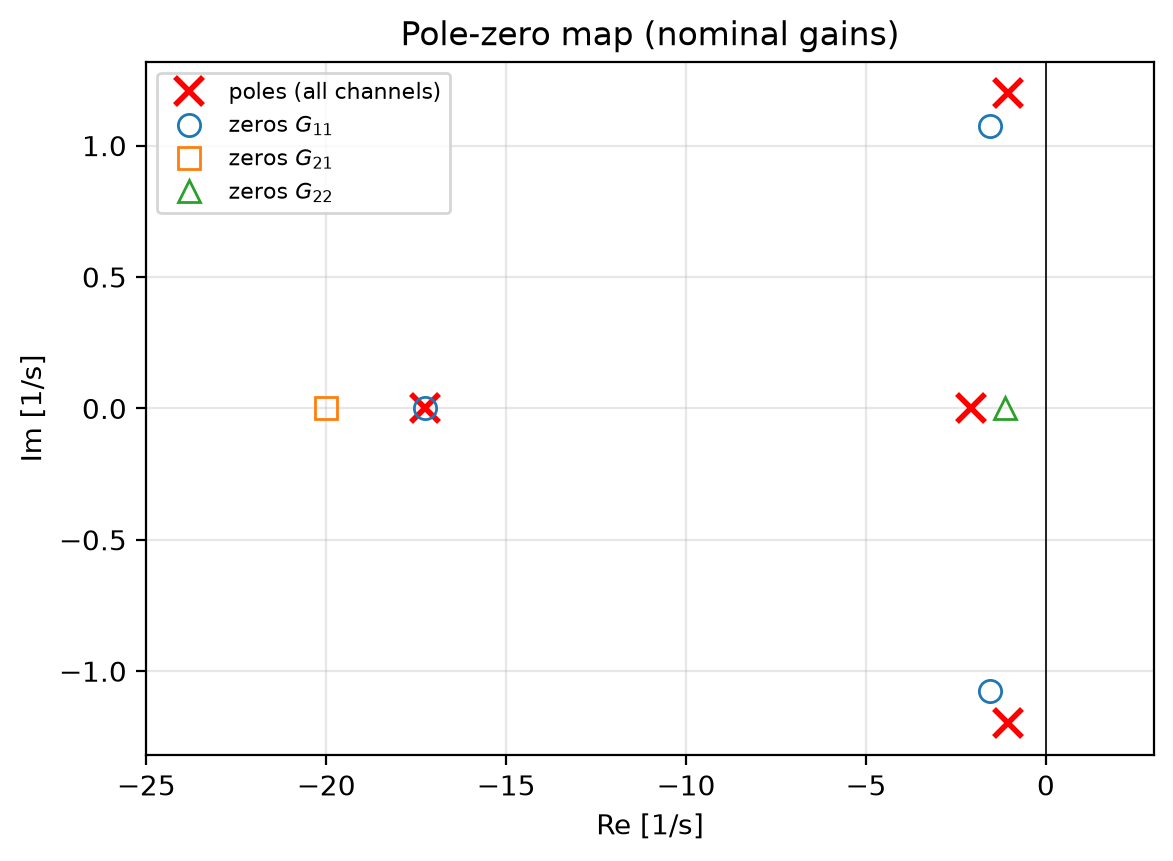
\includegraphics[width=0.85\columnwidth]{fig_polezero.png}
\caption{Polos ($\times$) y ceros ($\circ,\square,\triangle$) con las ganancias nominales.}\label{fig:pz}
\end{figure}

La ganancia est\'atica $G(0)$ (valor final ante una entrada unitaria) admite cuatro lecturas f\'isicas:
\begin{equation}
G(0)=\begin{bmatrix}0{,}046&-8{,}98\\0{,}0018&1{,}040\end{bmatrix}.
\end{equation}
$G_{22}(0)=1{,}04$, pedir $5^\circ$ termina en $5{,}2^\circ$, casi sin error, $G_{12}(0)=-8{,}98$, inclinar el cohete 1 rad resta casi 9 m/s$^2$ de aceleraci\'on axial (gravedad; se verific\'o a mano, $-c_\theta\tau_m\,G_{22}(0)/(1+K_1k_a)=-8{,}98$), $G_{11}(0)=0{,}046$, un escal\'on unitario de empuje da una aceleraci\'on final peque\~na porque $k_a$ es peque\~no, $G_{21}(0)=0{,}0018$, acelerar casi no inclina al cohete en estado estable, en t\'erminos de los escalones de prueba, 10~\% de empuje produce $0{,}459$ m/s$^2$ (unos 0,05 g) y 5$^\circ$ de comando producen $5{,}20^\circ$ de cabeceo y una aceleraci\'on acoplada de $-0{,}78$ m/s$^2$.


\subsection*{Estabilidad y papel de la tobera}
Un cohete estable es el que, despu\'es de un golpe, regresa a la calma, todos los polos con parte real negativa, pero el cohete es aerodin\'amicamente inestable ($\mu>0$), as\'i que la estabilidad depende de que la tobera sea lo bastante fuerte, el polinomio caracter\'istico $D(p)=a_4p^4+\dots+a_0$ es una funci\'on de $K_1$ y $K_2$, y el criterio de Routh--Hurwitz da condiciones sobre sus coeficientes (todos positivos y $\Delta_3=a_3a_2a_1-a_4a_1^2-a_3^2a_0>0$) que garantizan estabilidad sin calcular polos.

\begin{figure}[!t]
\centering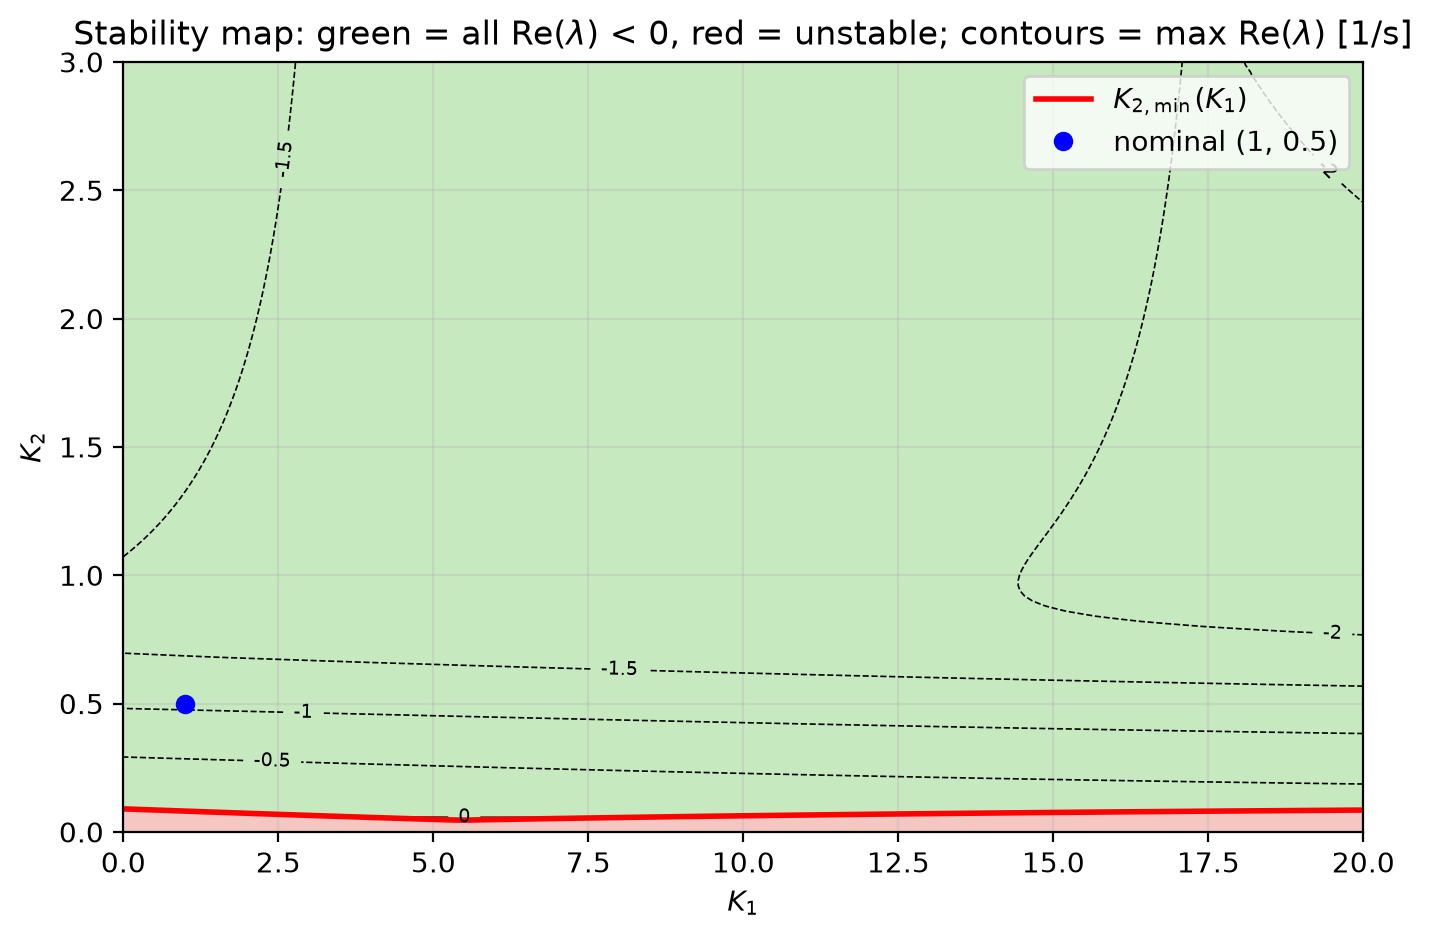
\includegraphics[width=\columnwidth]{fig_stab_map.png}
\caption{Mapa de estabilidad en el plano $(K_1,K_2)$, verde, estable; rojo, inestable, las l\'ineas son el mayor $\mathrm{Re}(\lambda)$ y la roja es $K_{2,\min}(K_1)$.}\label{fig:stab}
\end{figure}

El resultado est\'a en la figura~\ref{fig:stab}, hay dos par\'ametros (los ejes) y una respuesta ``estable o inestable'', por lo que un mapa 2D muestra de un vistazo toda la regi\'on segura, existe un $K_2$ m\'inimo, entre $0{,}046$ y $0{,}085$ para $K_1\in[0{,}5;20]$, casi todo el plano es estable; basta $K_2\gtrsim0{,}09$, las curvas de nivel (qu\'e tan estable es el cohete) son casi horizontales, $K_2$ manda en la rapidez con que el cohete se asienta y $K_1$ influye muy poco en la estabilidad, f\'isicamente, la inestabilidad viene de $\mu$, que act\'ua en la rotaci\'on, y la \'unica pieza que la combate es el servo, controlado por $K_2$; $K_1$ pertenece al canal del motor, que ya era estable, el nominal $(1;0{,}5)$ queda en la curva de $-1$ s$^{-1}$, su modo m\'as lento se apaga con tiempo caracter\'istico de aproximadamente 1 s.

\begin{figure}[!t]
\centering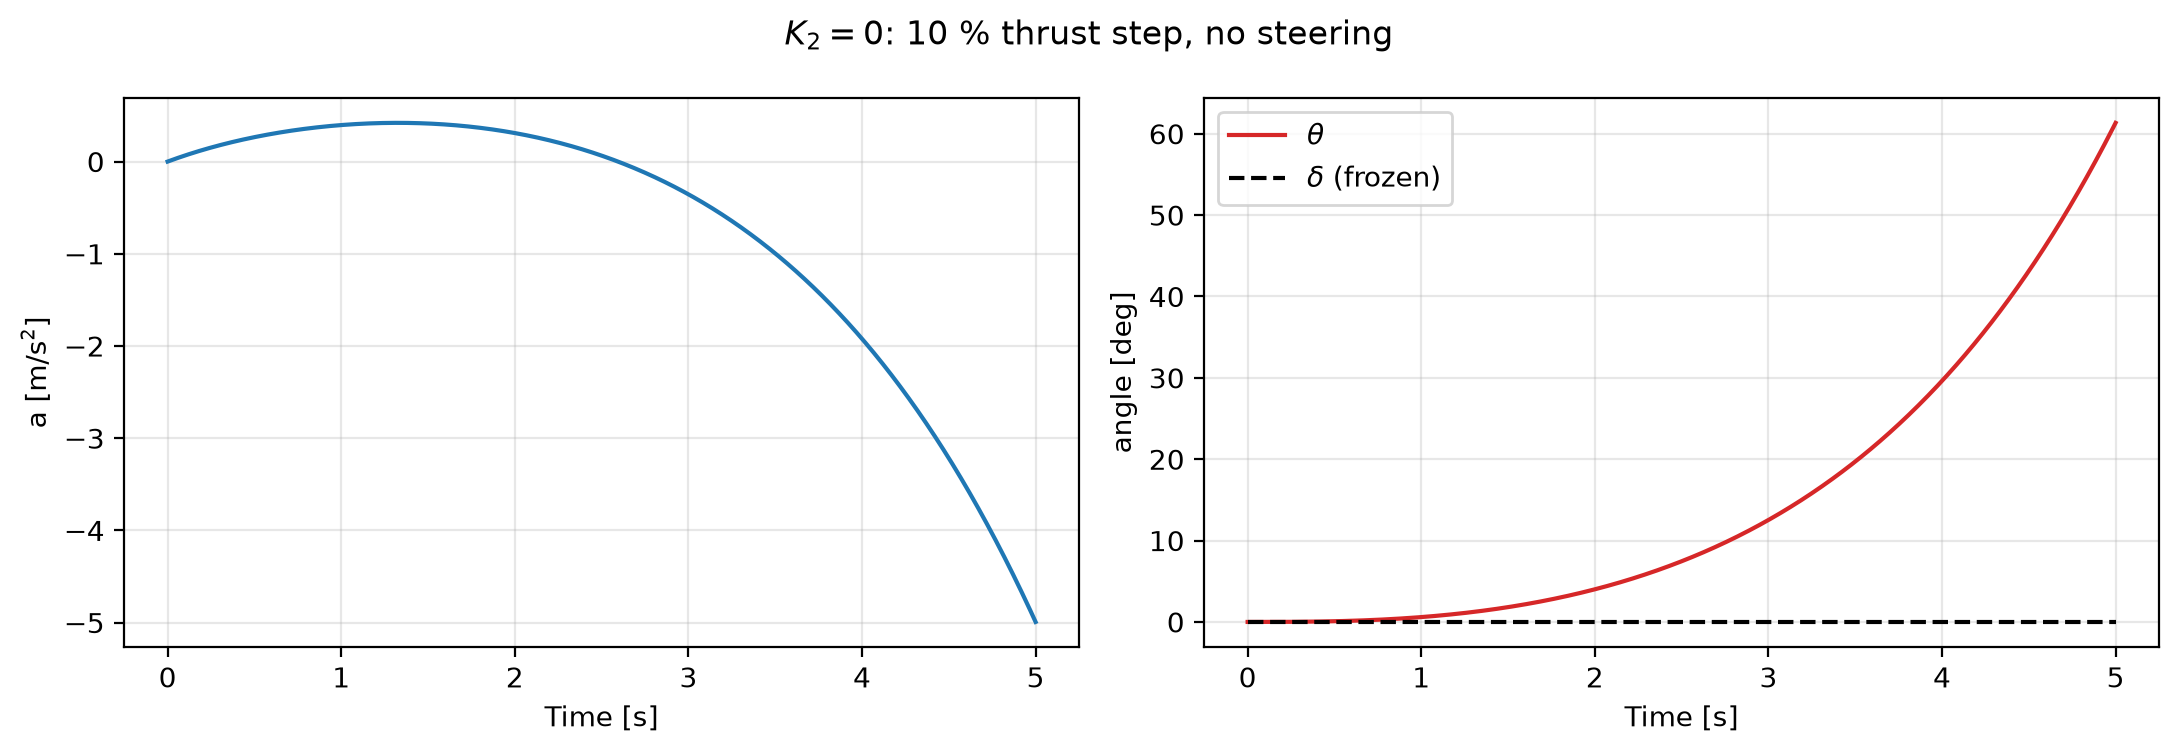
\includegraphics[width=\columnwidth]{fig_k2_0_unstable.png}
\caption{Caso $K_2=0$ con un escal\'on de 10~\% de empuje, $\theta$ crece y $\delta$ queda congelada en 0.}\label{fig:k20}
\end{figure}

Con $K_2=0$ el servo se desconecta y la tobera nunca se mueve, aparece un polo en $+0{,}557$ s$^{-1}$, de modo que el \'angulo se multiplica por $e^{0{,}557}\approx1{,}75$ cada segundo (figura~\ref{fig:k20}), $\theta$ sube hasta unos $60^\circ$ en 5 s, y la aceleraci\'on, que empieza a subir porque el motor s\'i responde a $u_1$, se vuelve negativa porque la inclinaci\'on creciente le resta aceleraci\'on por $-c_\theta\theta$, sin direcci\'on, el aire (que act\'ua con $\mu$) voltea al cohete.


\subsection*{Respuesta a se\~nales de prueba y efecto de las ganancias}
Para conocer un cohete se le ``golpea'' de distintas formas y se observa c\'omo reacciona, se usaron tres se\~nales (con entrada unitaria, solo para el an\'alisis lineal), un \emph{pulso} $H(t)-H(t-5)$, que es una maniobra que se enciende 5 s y se apaga; una \emph{senoide} $\sin t$, como una vibraci\'on peri\'odica o corrientes de aire; y un \emph{impulso} $K\delta(t)$, una r\'afaga, cada una se aplic\'o a $u_1$ solo, a $u_2$ solo y a ambas, para separar la causa, siempre se grafica $y(t)=[a,\theta]$ contra el tiempo, porque es lo que ver\'ia un ingeniero en la telemetr\'ia.

\begin{figure*}[!t]
\centering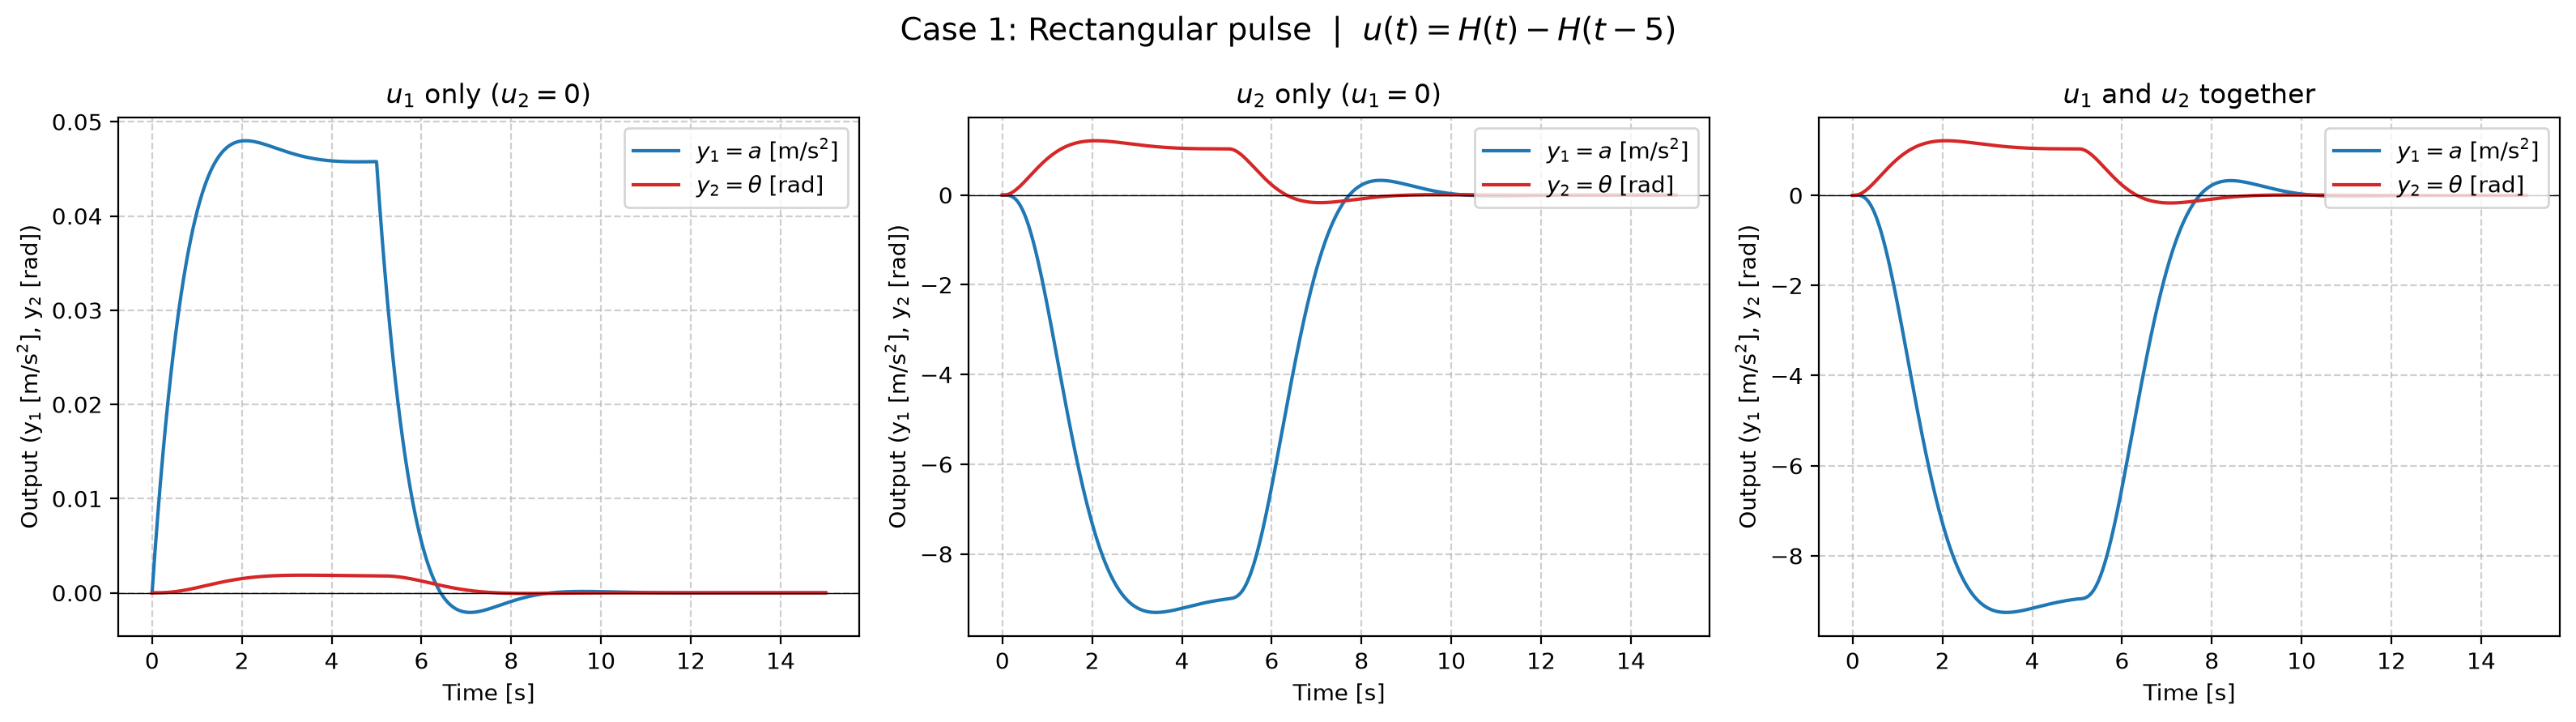
\includegraphics[width=0.92\textwidth]{fig_q7_pulse.png}
\caption{Respuesta al pulso rectangular de 5 s, para $u_1$ solo, $u_2$ solo y ambas.}\label{fig:pulse}
\end{figure*}

\textbf{Pulso.} Con $u_1$ solo, $a$ sube a unos $0{,}048$ m/s$^2$ en 2 s y se mantiene mientras dura el pulso, mientras que $\theta$ casi no se mueve ($0{,}002$ rad); cuando el pulso termina, $a$ regresa a cero en unos 2 s, con $u_2$, $\theta$ sube a $1{,}1$ rad y se queda cerca de 1 rad, mientras $a$ \emph{baja} a unos $-9$ m/s$^2$, es el acoplamiento por gravedad, $G_{12}(0)\approx-8{,}98$, al terminar el pulso el servo y el controlador enderezan al cohete y $a$ rebota levemente ($+0{,}3$) antes de asentarse, los valores en que se mantienen las curvas durante el pulso son la ganancia est\'atica $G(0)$, y todas regresan a cero tras el pulso (estabilidad).

\begin{figure*}[!t]
\centering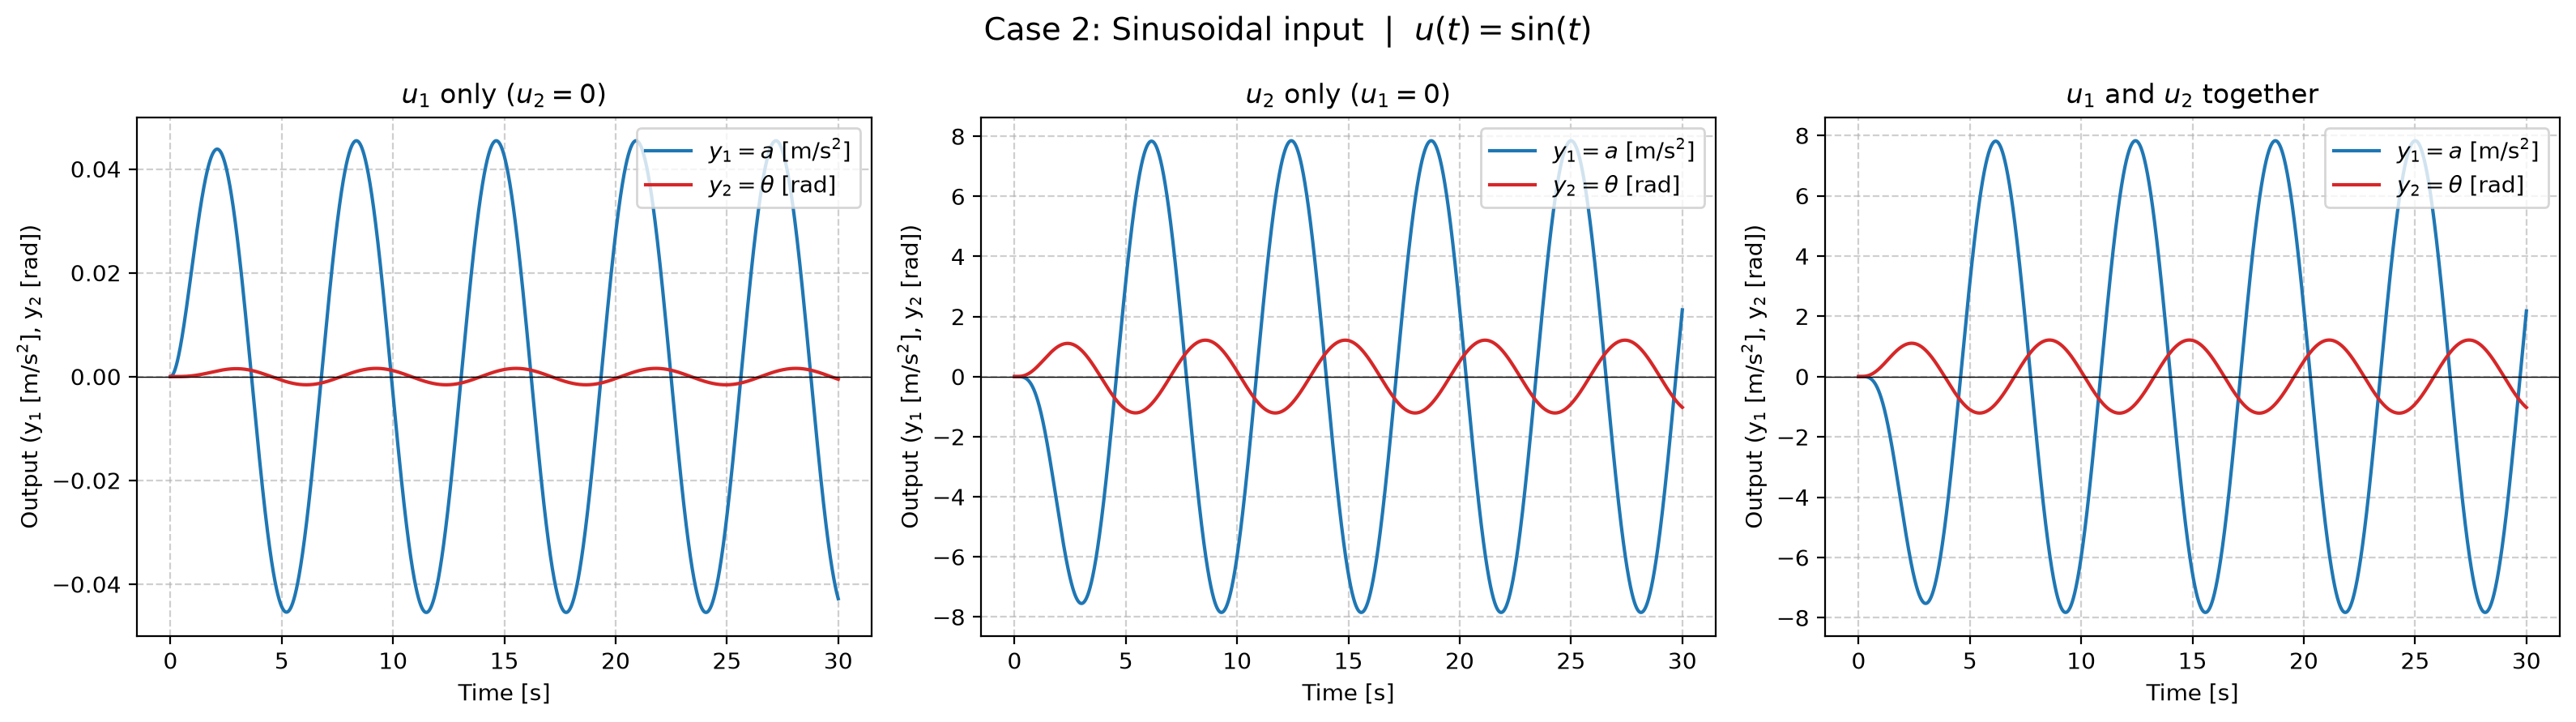
\includegraphics[width=0.92\textwidth]{fig_q7_sine.png}
\caption{Respuesta a la entrada senoidal $\sin t$ ($\omega=1$ rad/s).}\label{fig:sine}
\end{figure*}

\textbf{Senoide.} Tras un breve transitorio las salidas oscilan a la misma frecuencia que la entrada (periodo $2\pi\approx6{,}3$ s) con amplitud constante, $a$ de $\pm0{,}045$ por $u_1$; $a\approx\pm7{,}8$ y $\theta\approx\pm1{,}2$ por $u_2$, es la base de la respuesta en frecuencia, un sistema estable responde a una senoide con otra senoide de la misma frecuencia, con otra amplitud y otro desfase, a 1 rad/s las amplitudes son aproximadamente las ganancias est\'aticas, porque 1 rad/s est\'a dentro del ancho de banda del cohete, que ronda los 2 rad/s.

\begin{figure*}[!t]
\centering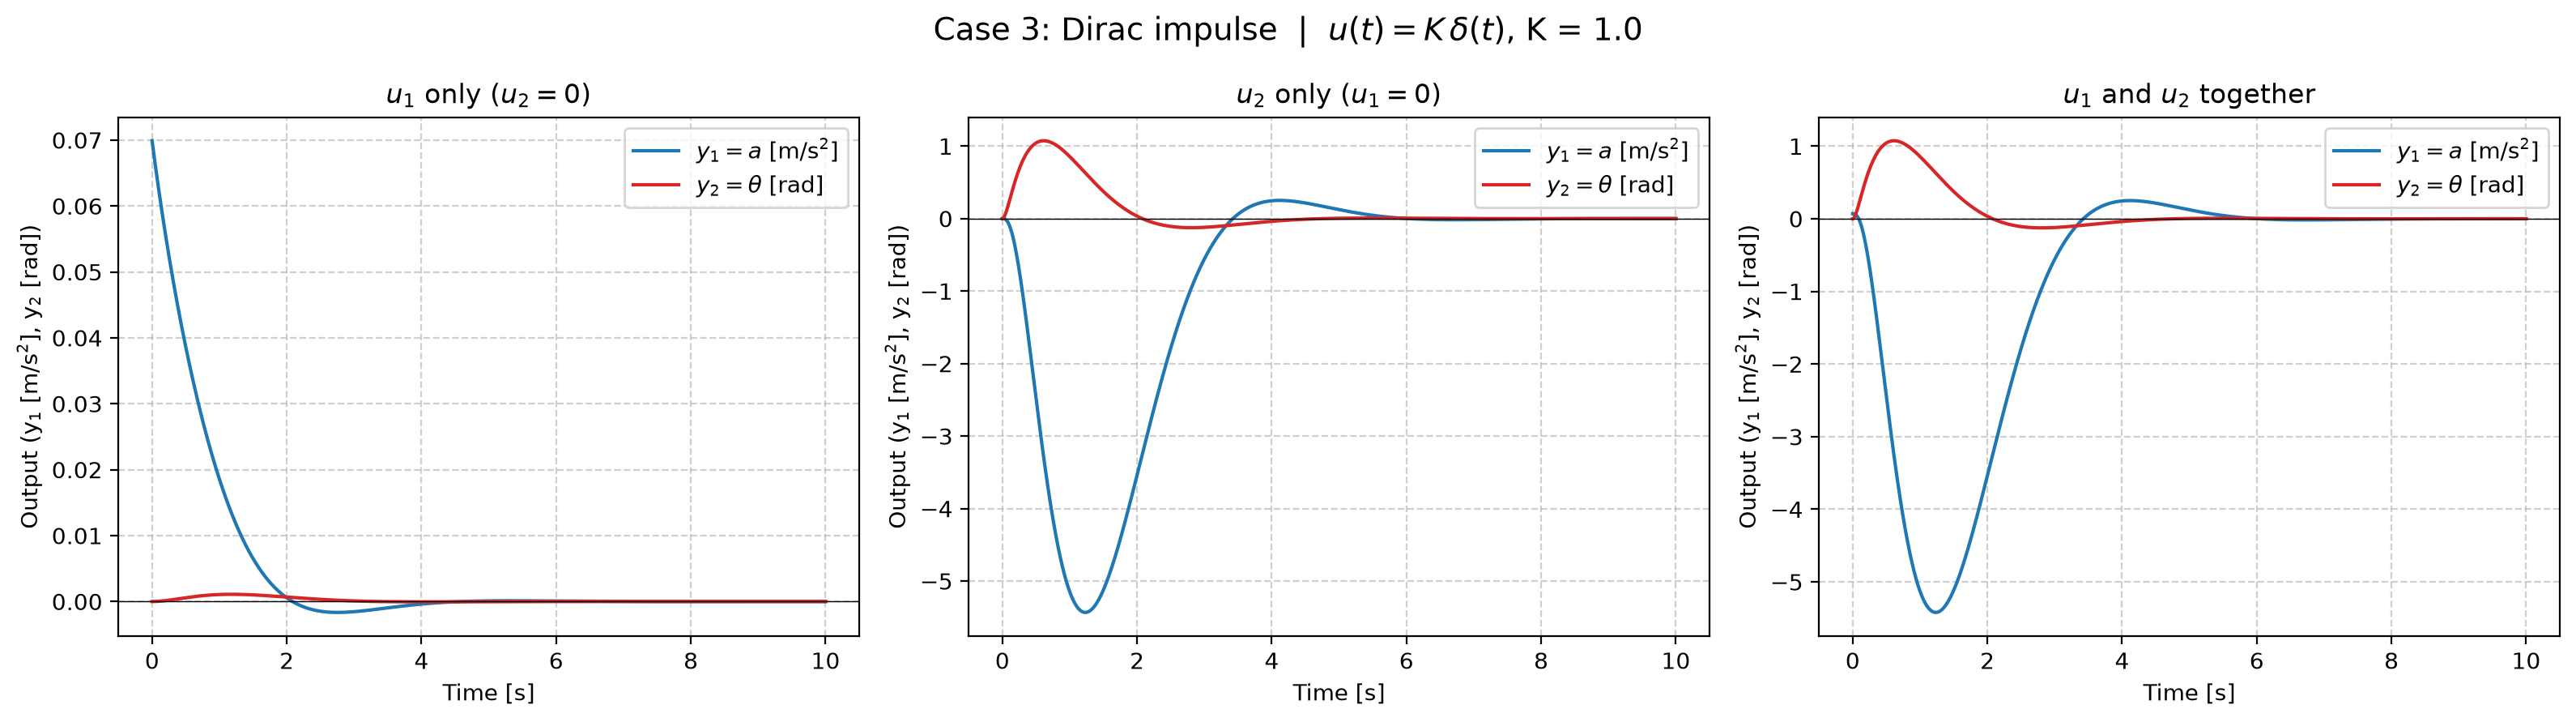
\includegraphics[width=0.92\textwidth]{fig_q7_impulse.png}
\caption{Respuesta al impulso (r\'afaga) $K\delta(t)$ con $K=1$.}\label{fig:impulse}
\end{figure*}

\textbf{Impulso.} Una r\'afaga se apaga sola en 5--6 s (figura~\ref{fig:impulse}), con $u_2$, $\theta$ sube a $1{,}1$ rad en 0,6 s y $a$ cae a $-5{,}4$ m/s$^2$ en 1,2 s; ambas regresan a cero con un rebote suave, un impulso excita todos los modos a la vez, y la forma en que se apaga es la huella de los polos, la envolvente decae como $e^{-1{,}07t}$ (polos lentos $-1{,}07\pm1{,}20j$) y el rebote es el efecto de su parte imaginaria; el polo r\'apido $-17{,}3$ se apaga en una d\'ecima de segundo y casi no se ve, con $u_1$ solo, la curva de $a$ empieza en $0{,}07$ m/s$^2$ de forma instant\'anea, que es $K_1k_a/\tau_m$, $u_1$ entra directo al estado $a$ (el \'unico canal con salto inicial, pues los dem\'as tienen tres o cuatro eslabones).

\begin{figure*}[!t]
\centering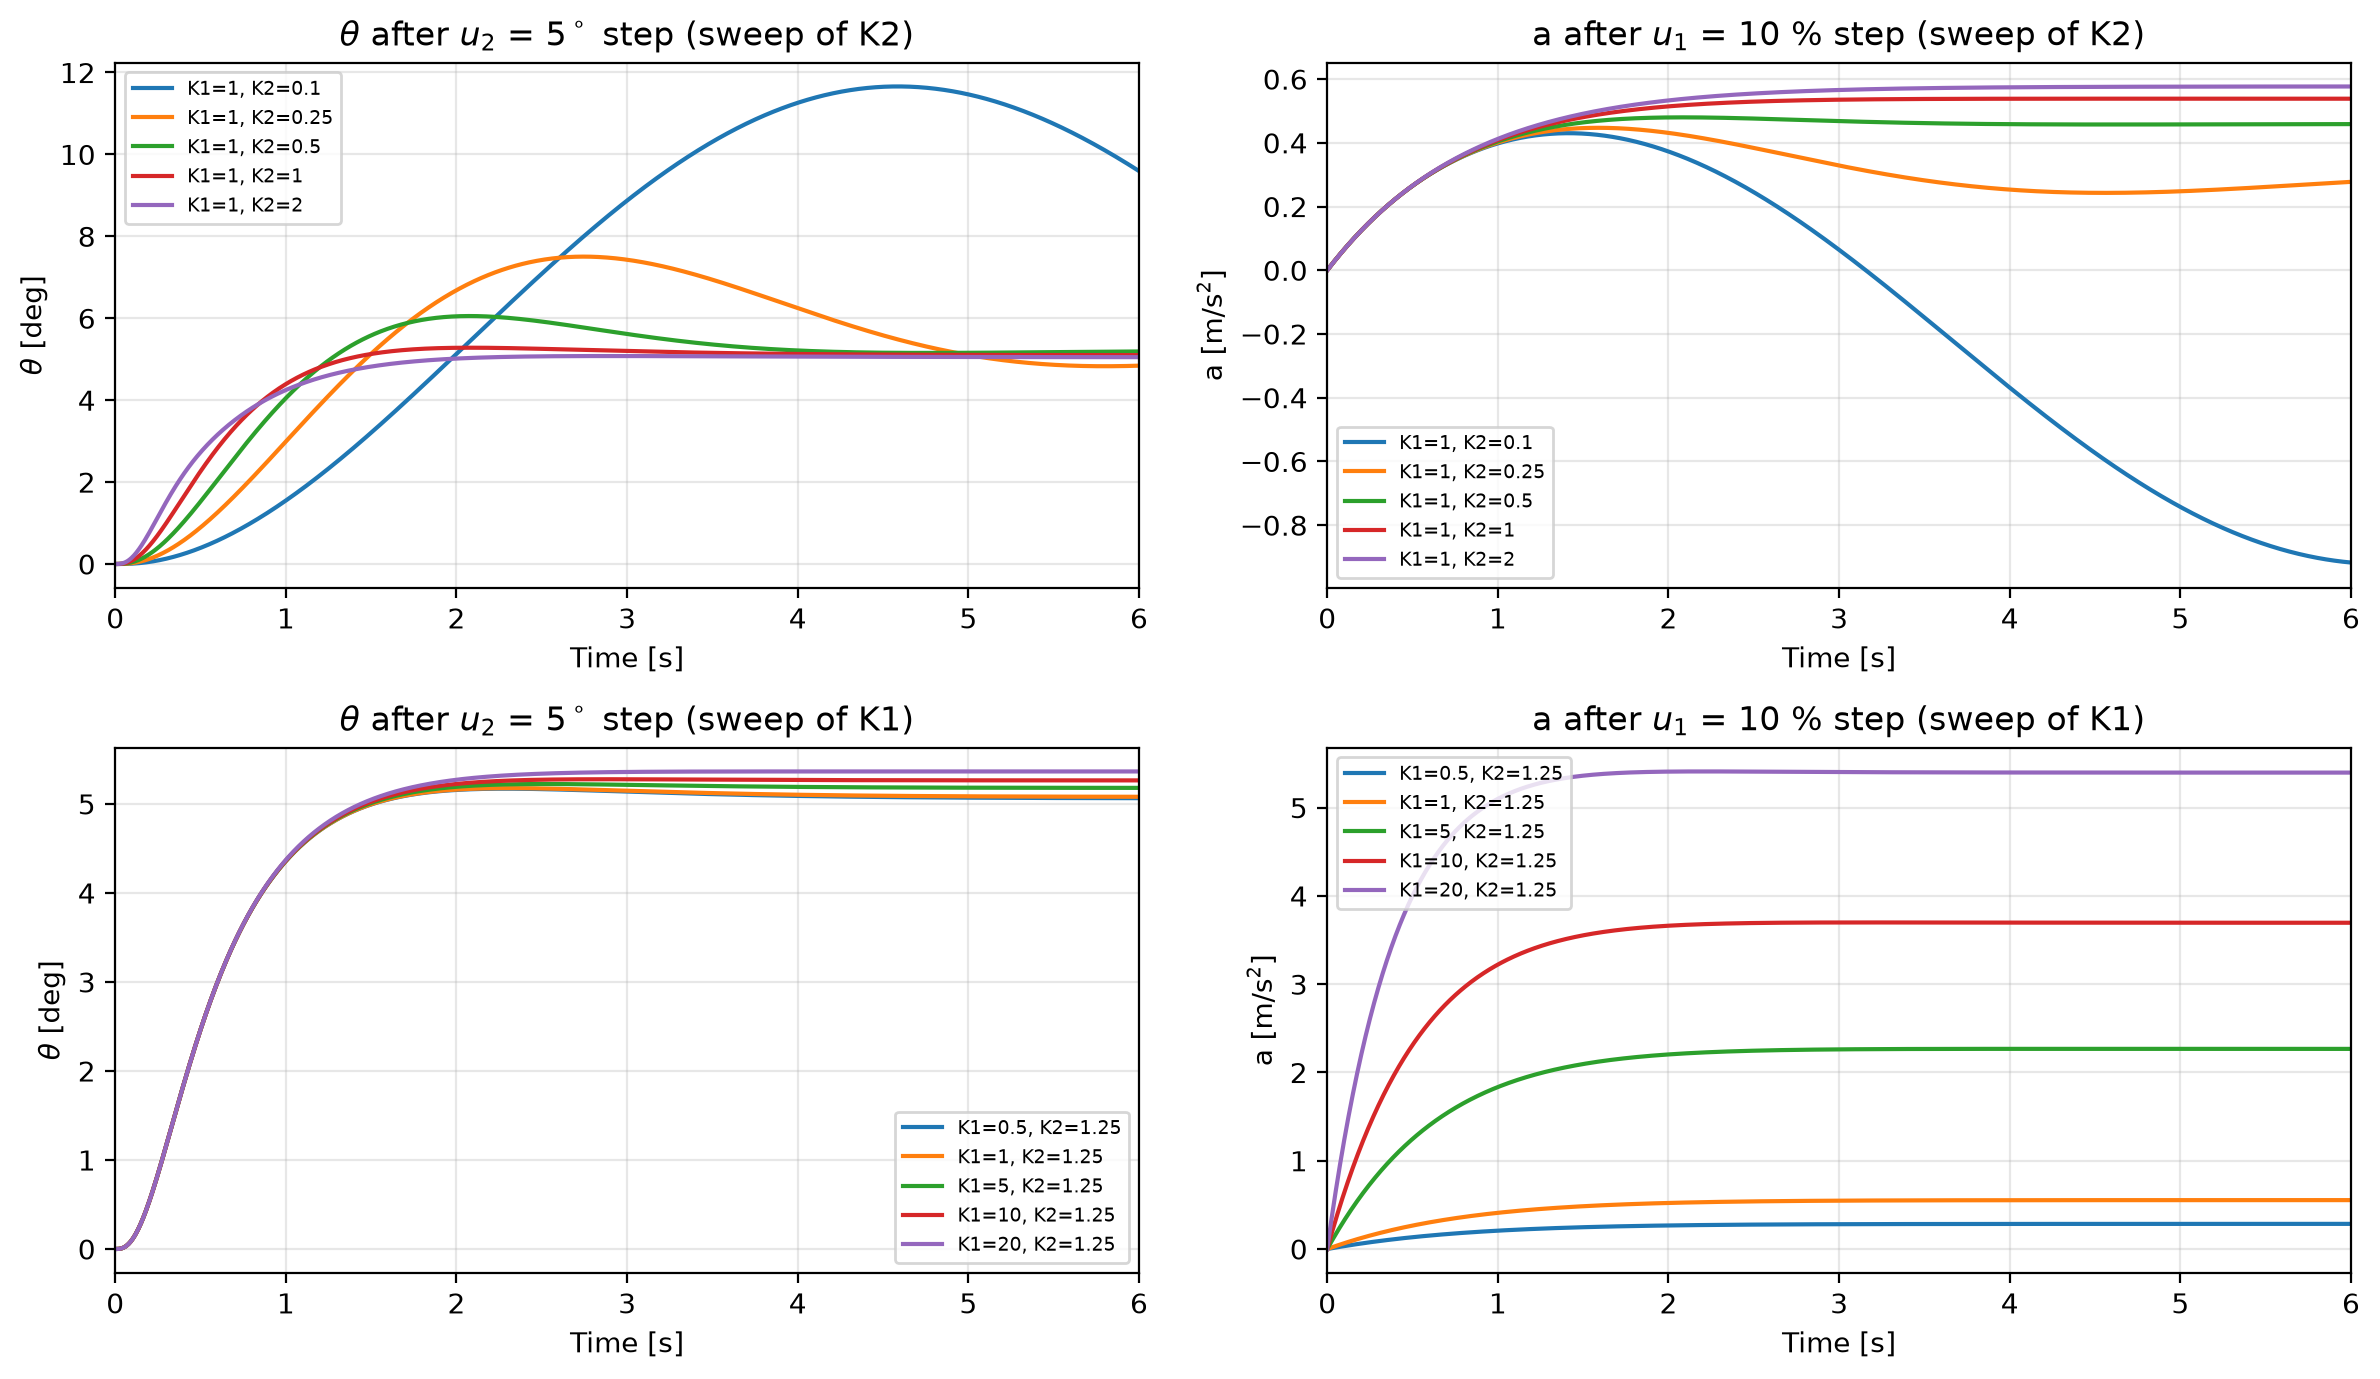
\includegraphics[width=0.8\textwidth]{fig_q7_gain_sweep.png}
\caption{Efecto de $K_2$ (arriba) y de $K_1$ (abajo) en la rapidez y la estabilidad.}\label{fig:sweep}
\end{figure*}

\textbf{Efecto de las ganancias.} La forma m\'as r\'apida de ver el efecto de una perilla es superponer una curva por ganancia (figura~\ref{fig:sweep}), arriba, con un escal\'on de $5^\circ$ en $u_2$, con $K_2=0{,}1$ el cohete se pasa hasta $11{,}7^\circ$ y tarda m\'as de 6 s en asentarse (la tobera casi no tiene fuerza para frenar); con $K_2=0{,}25$ llega a $7{,}5^\circ$ (50~\% de sobrepaso); con $K_2\ge1$ sube r\'apido y limpio, abajo, con $K_2=1{,}25$ fijo, $\theta$ casi no depende de $K_1$, pero la aceleraci\'on final s\'i, de $0{,}3$ m/s$^2$ con $K_1=0{,}5$ a $5{,}4$ m/s$^2$ con $K_1=20$ para el mismo 10~\% de empuje, cada ganancia tiene su trabajo, $K_2$ gobierna la actitud (rapidez y amortiguamiento del giro) y $K_1$ gobierna cu\'anta aceleraci\'on se logra con el comando de empuje.


\subsection*{Acoplamiento entre canales}
\textbf{Cu\'anto se acoplan los canales.} Como $a$ y $\theta$ no se pueden comparar directamente (m/s$^2$ contra rad), se mide cada desviaci\'on cruzada respecto a la salida principal del otro canal, con los escalones de $u_1=10$~\% y $u_2=5^\circ$ (figura~\ref{fig:coupling}), con las ganancias nominales:
\begin{itemize}
  \item Un escal\'on en $u_2$ lleva a $\theta$ a $5{,}20^\circ$, pero la aceleraci\'on cae hasta $-0{,}81$ m/s$^2$ y se queda en $-0{,}78$, la inclinaci\'on le quita casi 0,8 m/s$^2$, comparado con los $0{,}459$ m/s$^2$ que da el 10~\% de empuje, el acoplamiento $u_2\to a$ es de \textbf{177~\%}, inclinar al cohete le quita m\'as aceleraci\'on de la que le da el empuje.
  \item Un escal\'on en $u_1$ lleva a $a$ a $0{,}459$ m/s$^2$ y desv\'ia a $\theta$ hasta $1{,}07^\circ$ (termina en $1{,}03^\circ$, por $k_\varepsilon$), frente a los $5{,}20^\circ$ de $u_2$, es \textbf{20,6~\%}.
\end{itemize}
El acoplamiento es asim\'etrico y el m\'as severo es $u_2\to a$, la gravedad ($c_\theta=9{,}81$, grande) hace fuerte ese camino, y $k_\varepsilon=0{,}12$ (peque\~no) hace d\'ebil el otro, con las ganancias nominales, el canal de actitud contamina al de aceleraci\'on.

\begin{figure}[!t]
\centering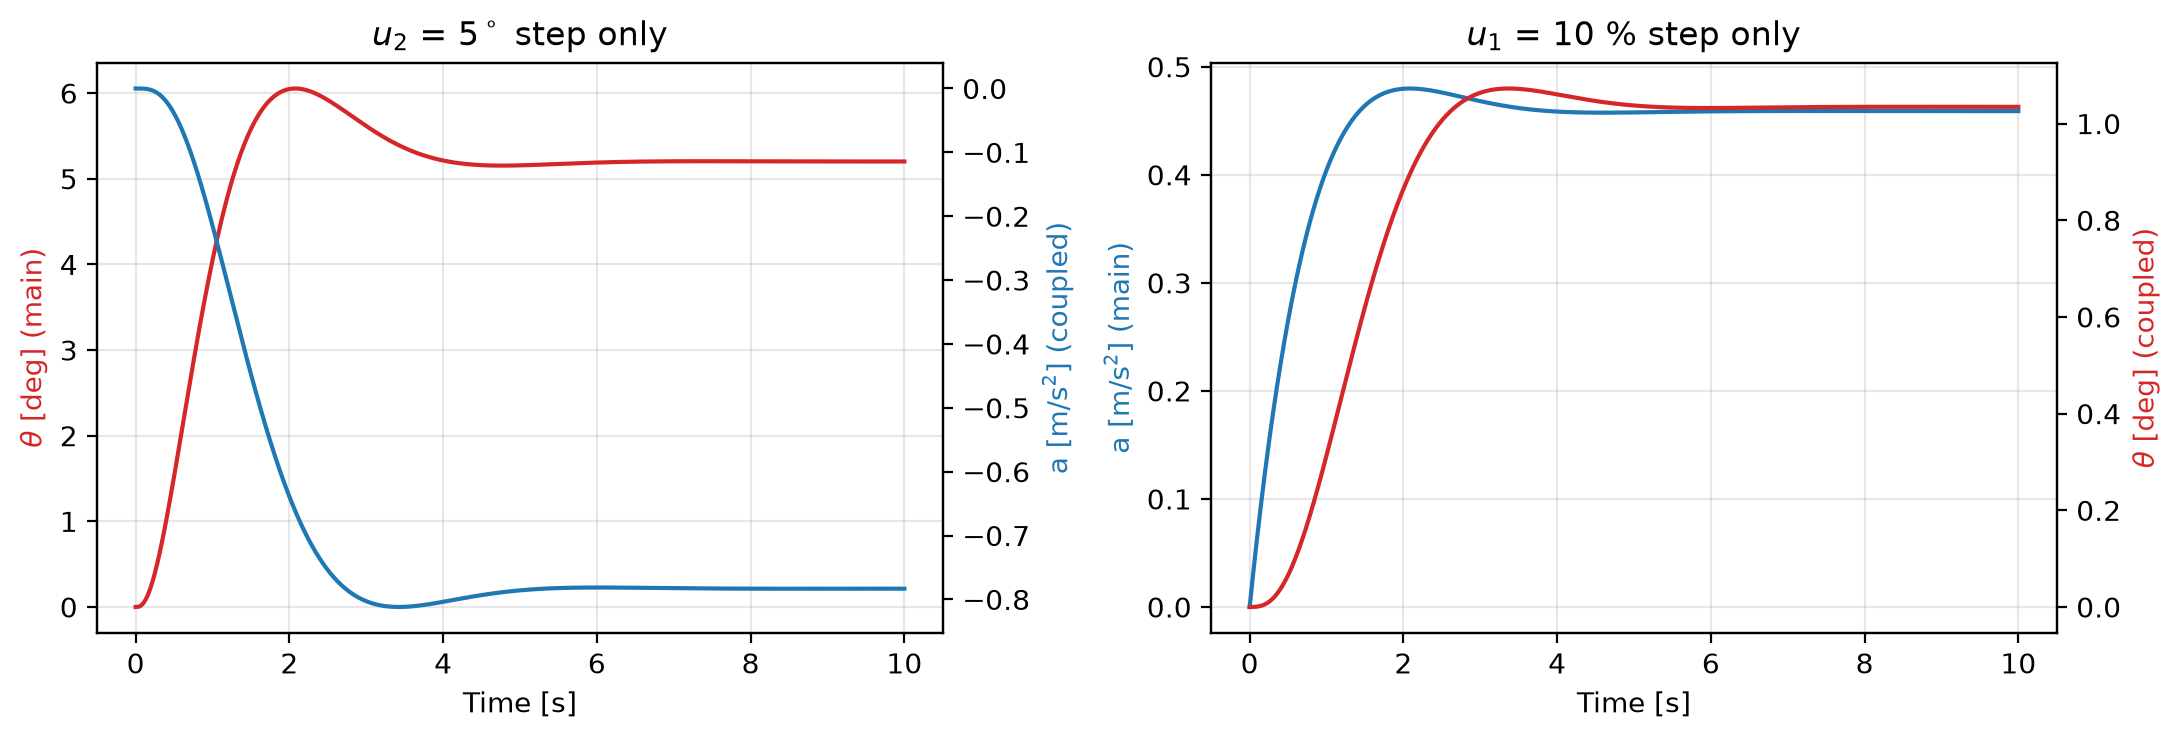
\includegraphics[width=\columnwidth]{fig_coupling.png}
\caption{Dos escalones, cada uno con la salida principal y la acoplada en dos ejes verticales.}\label{fig:coupling}
\end{figure}

Los porcentajes dependen de las ganancias a trav\'es de $G(0)$ (tabla~\ref{tab:acople}), subir $K_1$ de 1 a 10 multiplica $G_{11}(0)$ por 7 y reduce $u_2\to a$ de 177~\% a 18~\%; pero el mayor empuje inclina m\'as al cohete por $k_\varepsilon$ y $u_1\to\theta$ sube a 133~\%, subir $K_2$ a $1{,}3$ hace que la tobera sujete mejor la inclinaci\'on y $u_1\to\theta$ cae a 7,6~\%, ning\'un extremo baja ambos a la vez, un par intermedio, $(4{,}5;1{,}3)$, da 30,5~\% y 28,3~\%.

\begin{table}[!t]
\centering\footnotesize\setlength{\tabcolsep}{2.5pt}
\caption{Acoplamiento para distintas ganancias.}\label{tab:acople}
\begin{tabular}{rr|rrrr|rr}
\toprule
$K_1$ & $K_2$ & $G_{11}$ & $G_{12}$ & $G_{21}$ & $G_{22}$ & $u_2\!\to\! a$ & $u_1\!\to\!\theta$\\
 & & \multicolumn{4}{c|}{(en $p=0$)} & [\%] & [\%]\\
\midrule
1 & 0,5 & 0,046 & $-8{,}98$ & 0,0018 & 1,040 & 176,9 & 20,6\\
10 & 0,5 & 0,325 & $-6{,}35$ & 0,0128 & 1,144 & 17,7 & 132,5\\
1 & 1,3 & 0,056 & $-8{,}76$ & 0,0007 & 1,015 & 137,4 & 7,6\\
4,5 & 1,3 & 0,210 & $-7{,}33$ & 0,0026 & 1,033 & 30,5 & 28,3\\
\bottomrule
\end{tabular}
\end{table}

Para ver c\'omo depende el acoplamiento de la rapidez de la maniobra se pasa a la respuesta en frecuencia.

\begin{figure*}[!t]
\centering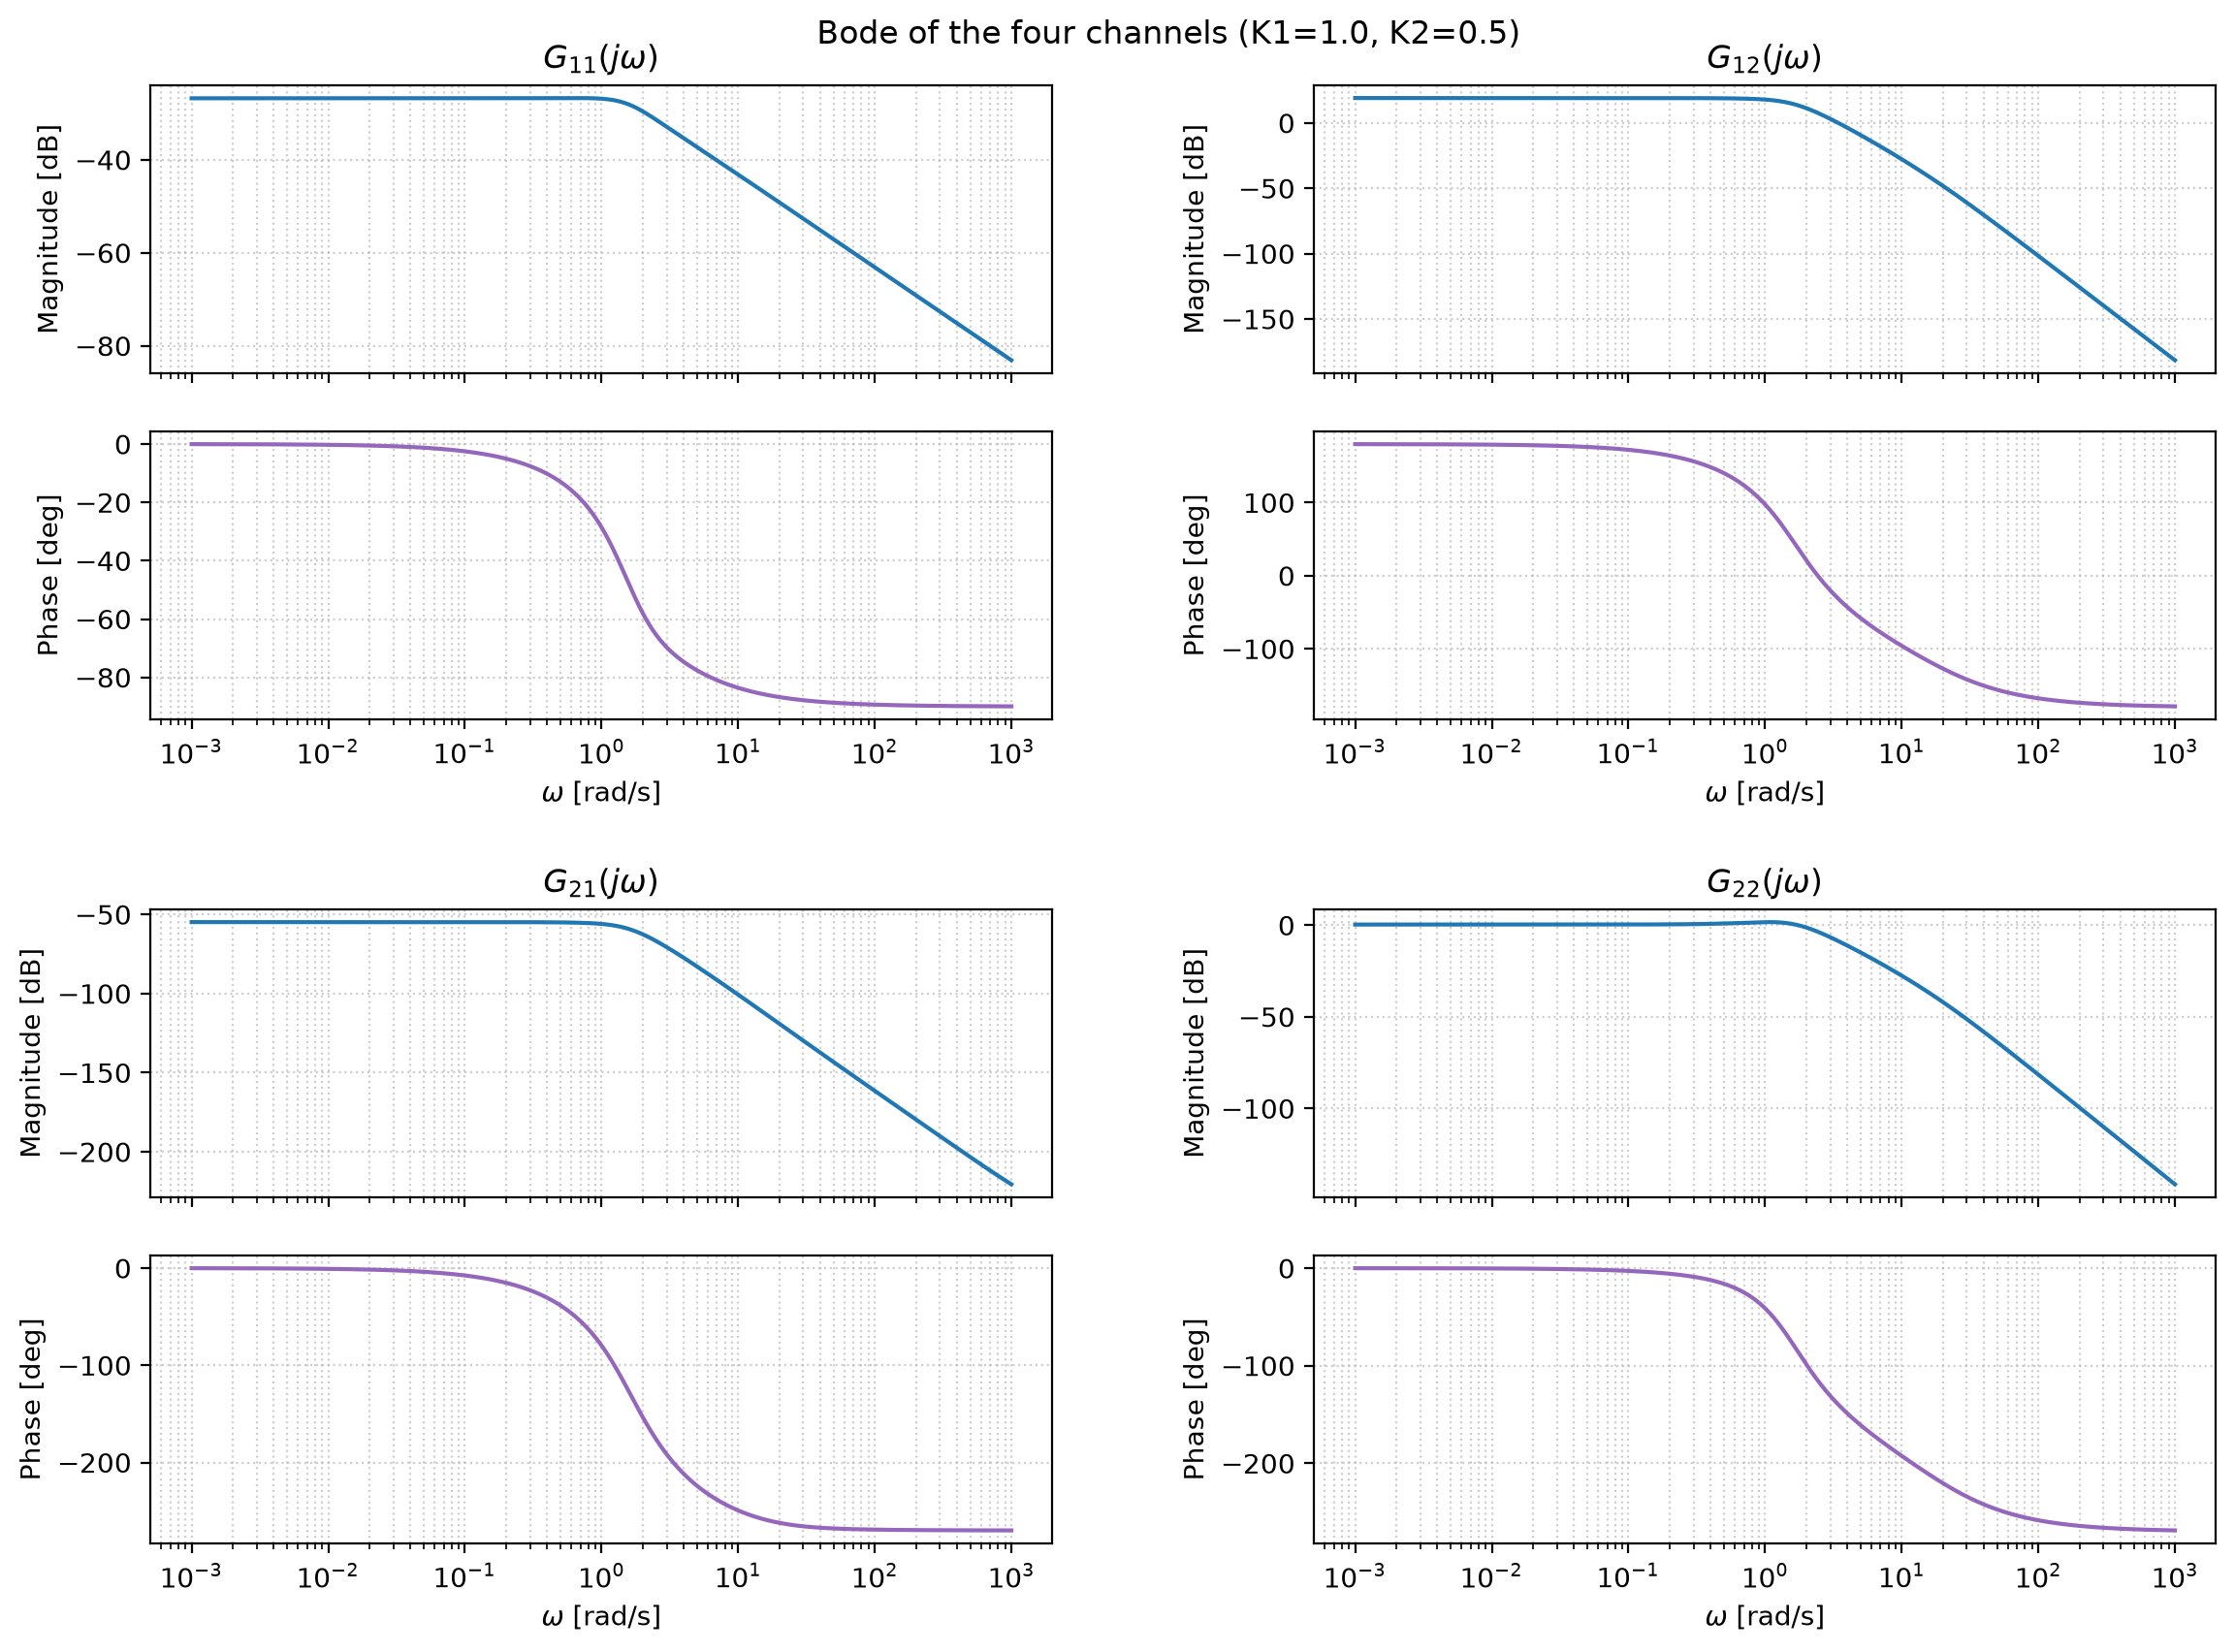
\includegraphics[width=0.88\textwidth]{fig_bode_2x2.png}
\caption{Diagrama de Bode de los cuatro canales con $(K_1,K_2)=(1;0{,}5)$, filas, salida ($a,\theta$); columnas, entrada ($u_1,u_2$).}\label{fig:bode}
\end{figure*}

El diagrama de Bode (figura~\ref{fig:bode}) muestra, para cada canal, la ganancia en decibeles (dB; $-20$ dB es una d\'ecima, $0$ dB es igual, $+20$ dB es diez veces) y el retraso de fase frente a la frecuencia, en escala logar\'itmica porque abarca seis \'ordenes de magnitud, todos los canales tienen una ``meseta'' a baja frecuencia, que es $G(0)$, $-27$ dB ($0{,}046$) en $G_{11}$, $0$ dB en $G_{22}$ (el cohete sigue la orden, con una peque\~na joroba cerca de 1--2 rad/s), $+19$ dB ($8{,}98$) en $G_{12}$ con fase inicial de $180^\circ$ (es el signo negativo, inclinar resta aceleraci\'on) y $-55$ dB ($0{,}0018$) en $G_{21}$, a frecuencias altas la magnitud cae con pendiente $-20\,r$ dB/d\'ecada, donde $r$ es el \emph{grado relativo} (n\'umero de polos menos n\'umero de ceros), $G_{11}$ tiene 4 polos y 3 ceros ($r=1$), $G_{21}$ y $G_{22}$ tienen 4 polos y 1 cero ($r=3$) y $G_{12}$ tiene 4 polos y ning\'un cero ($r=4$), f\'isicamente, cada polo sin cero que lo compense es un eslab\'on m\'as entre la orden y la salida (un retraso del motor, del servo o el giro) que a frecuencias altas atenúa 20 dB por d\'ecada y suma $-90^\circ$ de fase; por eso la fase final tiende a $-90^\circ$ en $G_{11}$ y a $-270^\circ$ en $G_{21}$ y $G_{22}$, las pendientes medidas, $-20{,}0$; $-79{,}9$; $-60{,}0$ y $-59{,}9$ dB/d\'ecada, coinciden con $-20r$, con m\'as eslabones la respuesta arranca m\'as lenta, por eso en el pulso $a$ casi no se mueve en el primer segundo cuando se manda $u_2$.

\begin{figure*}[!t]
\centering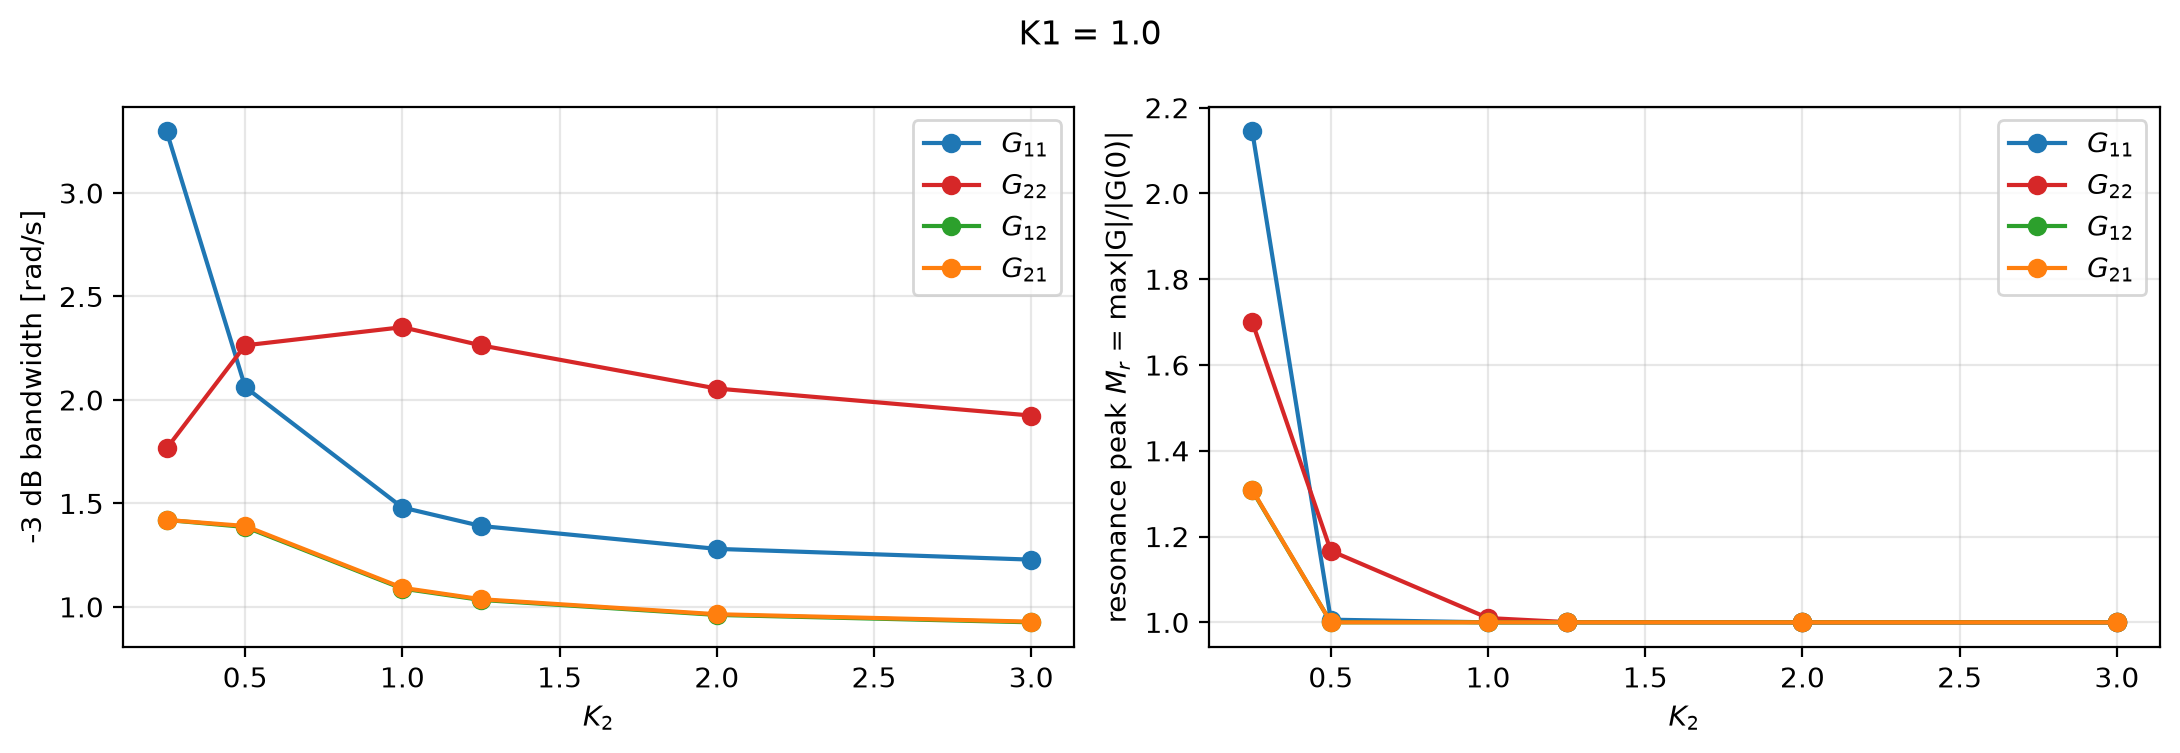
\includegraphics[width=0.8\textwidth]{fig_bw_vs_k2.png}
\caption{Ancho de banda (izquierda) y pico de resonancia (derecha) al subir $K_2$, con $K_1=1$.}\label{fig:bw}
\end{figure*}

\textbf{Ancho de banda y resonancia.} El ancho de banda (BW) es la frecuencia hasta la cual el canal sigue bien una orden (donde la magnitud cae 3 dB) y el pico de resonancia $M_r$ mide la amplificaci\'on m\'axima respecto a baja frecuencia ($M_r>1$ indica tendencia a oscilar), al subir $K_2$ (figura~\ref{fig:bw}), con $K_2=0{,}25$ hay resonancia clara ($M_r=2{,}15$ en $G_{11}$ y $1{,}70$ en $G_{22}$) y desde $K_2\ge0{,}5$ todos bajan a $\approx1$, $K_2$ amortigua, el BW de $G_{22}$ (actitud) es mejor cerca de $K_2\approx1$ (2,35 rad/s) y luego baja un poco, mientras que el de $G_{11}$ (aceleraci\'on) baja de 3,3 a 1,2 rad/s al subir $K_2$, una tobera m\'as fuerte endereza antes al cohete pero tambi\'en recorta la aceleraci\'on axial por la gravedad, es un compromiso real del modelo, por encima de unos 2 rad/s el cohete no sigue \'ordenes; corregir m\'as r\'apido solo gasta tobera.

\begin{figure}[!t]
\centering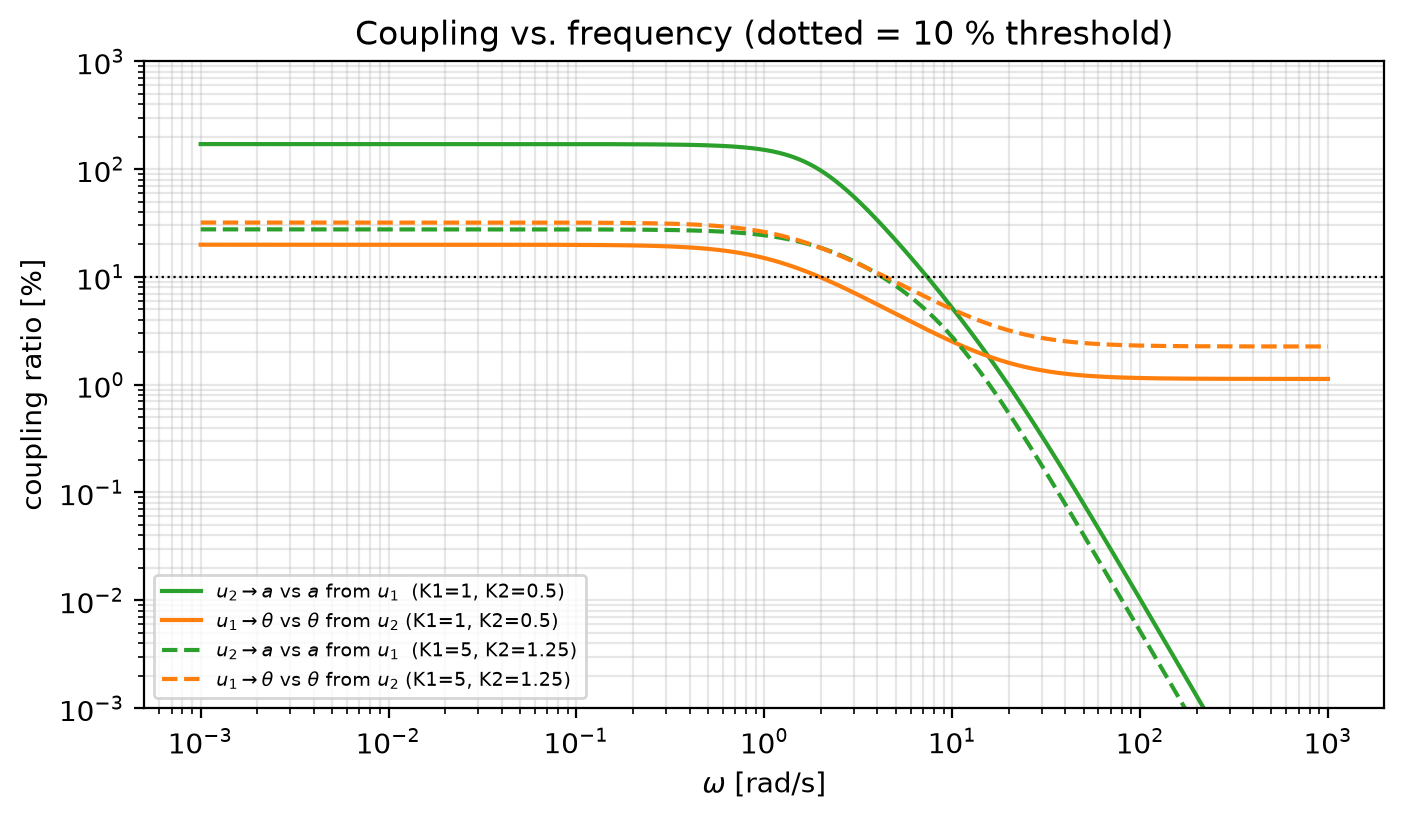
\includegraphics[width=\columnwidth]{fig_coupling_ratio.png}
\caption{Acoplamiento (\%) frente a la frecuencia; l\'inea punteada, umbral de 10~\%.}\label{fig:ratio}
\end{figure}

\textbf{¿Cu\'ando tratarlos como independientes?} La figura~\ref{fig:ratio} compara $|G_{12}|$ contra $|G_{11}|$ y $|G_{21}|$ contra $|G_{22}|$ (con los mismos escalones), las curvas son planas a baja frecuencia (el acoplamiento est\'atico de $\sim170$~\% y 20~\%) y caen al subir la frecuencia, con $(1;0{,}5)$, $u_2\to a$ supera 10~\% hasta 7,35 rad/s y $u_1\to\theta$ hasta 1,96 rad/s, con $(5;1{,}25)$, $u_2\to a$ baja a 28~\% pero $u_1\to\theta$ sube a 32~\% (las ganancias nuevas reparten el acoplamiento de forma m\'as pareja) y ambos son menores a 10~\% pasados unos 4 rad/s, cuando el comando var\'ia r\'apido (frecuencias mayores a unos 5 rad/s) los dos canales se pueden tratar casi como independientes; cuando var\'ia despacio, hay que considerar al cohete como un solo sistema MIMO.


\subsection*{Observabilidad y controlabilidad}
El cohete tiene cuatro estados pero solo se miden dos ($a$ y $\theta$); los otros, $\omega$ y $\delta$, no, ¿se pueden deducir de los sensores?, si s\'i, el sistema es \emph{observable}, importa porque el controlador usa $\omega$ en $v_2=K_2(u_2-\theta-\lambda\omega)$, cambiar de sensores no cambia el cohete (misma $A$, mismos polos), solo cambia la matriz $C$, o sea lo que se ve, con solo el aceler\'ometro $C=[1\;0\;0\;0]$; con solo la IMU $C=[0\;1\;0\;0]$; con ambos, la nominal; y si adem\'as se registra $\omega$ para monitorear cargas estructurales, se a\~nade la fila $[0\;0\;1\;0]$.

La observabilidad se verifica con el rango de $O=[C;CA;CA^2;CA^3]$ (rango 4 = observable)~\cite{nise}, adem\'as se usa $\sigma_{\min}(O)$, el valor singular m\'as peque\~no, que dice \emph{qu\'e tan bien}, cerca de cero es observable en teor\'ia pero muy sensible al ruido, con cualquier juego de sensores el rango es 4, pero la calidad difiere (tabla~\ref{tab:obs}), con solo $\theta$ el sistema es 45 veces m\'as fr\'agil que con $a$, como los estados tienen unidades distintas, $\sigma_{\min}$ sirve para comparar sensores entre s\'i, no como valor absoluto.

\begin{table}[!t]
\centering\small
\caption{Observabilidad seg\'un los sensores.}\label{tab:obs}
\begin{tabular}{lcc}
\toprule
Sensores & Rango de $O$ & $\sigma_{\min}(O)$\\
\midrule
solo $a$ & 4 & 0,993\\
solo $\theta$ & 4 & 0,026\\
$a$ y $\theta$ & 4 & 1,172\\
$a$, $\theta$ y $\omega$ & 4 & 1,34\\
\bottomrule
\end{tabular}
\end{table}

La causa es el propio acoplamiento, el aceler\'ometro \emph{oye} la inclinaci\'on por la gravedad ($-c_\theta\theta$ en $\dot a$), un camino fuerte, mientras que la IMU solo ve el empuje por $k_\varepsilon=0{,}12$, un camino d\'ebil, sin acoplamiento el cohete ser\'ia opaco, sin gravedad ($c_\theta=0$) con solo el aceler\'ometro el rango cae a 1 y sin desalineaci\'on ($k_\varepsilon=0$) con solo la IMU cae a 3, en un sistema no observable, un modo inestable podr\'ia crecer sin que los sensores lo vean y la computadora corregir\'ia con un estado equivocado.

\begin{figure*}[!t]
\centering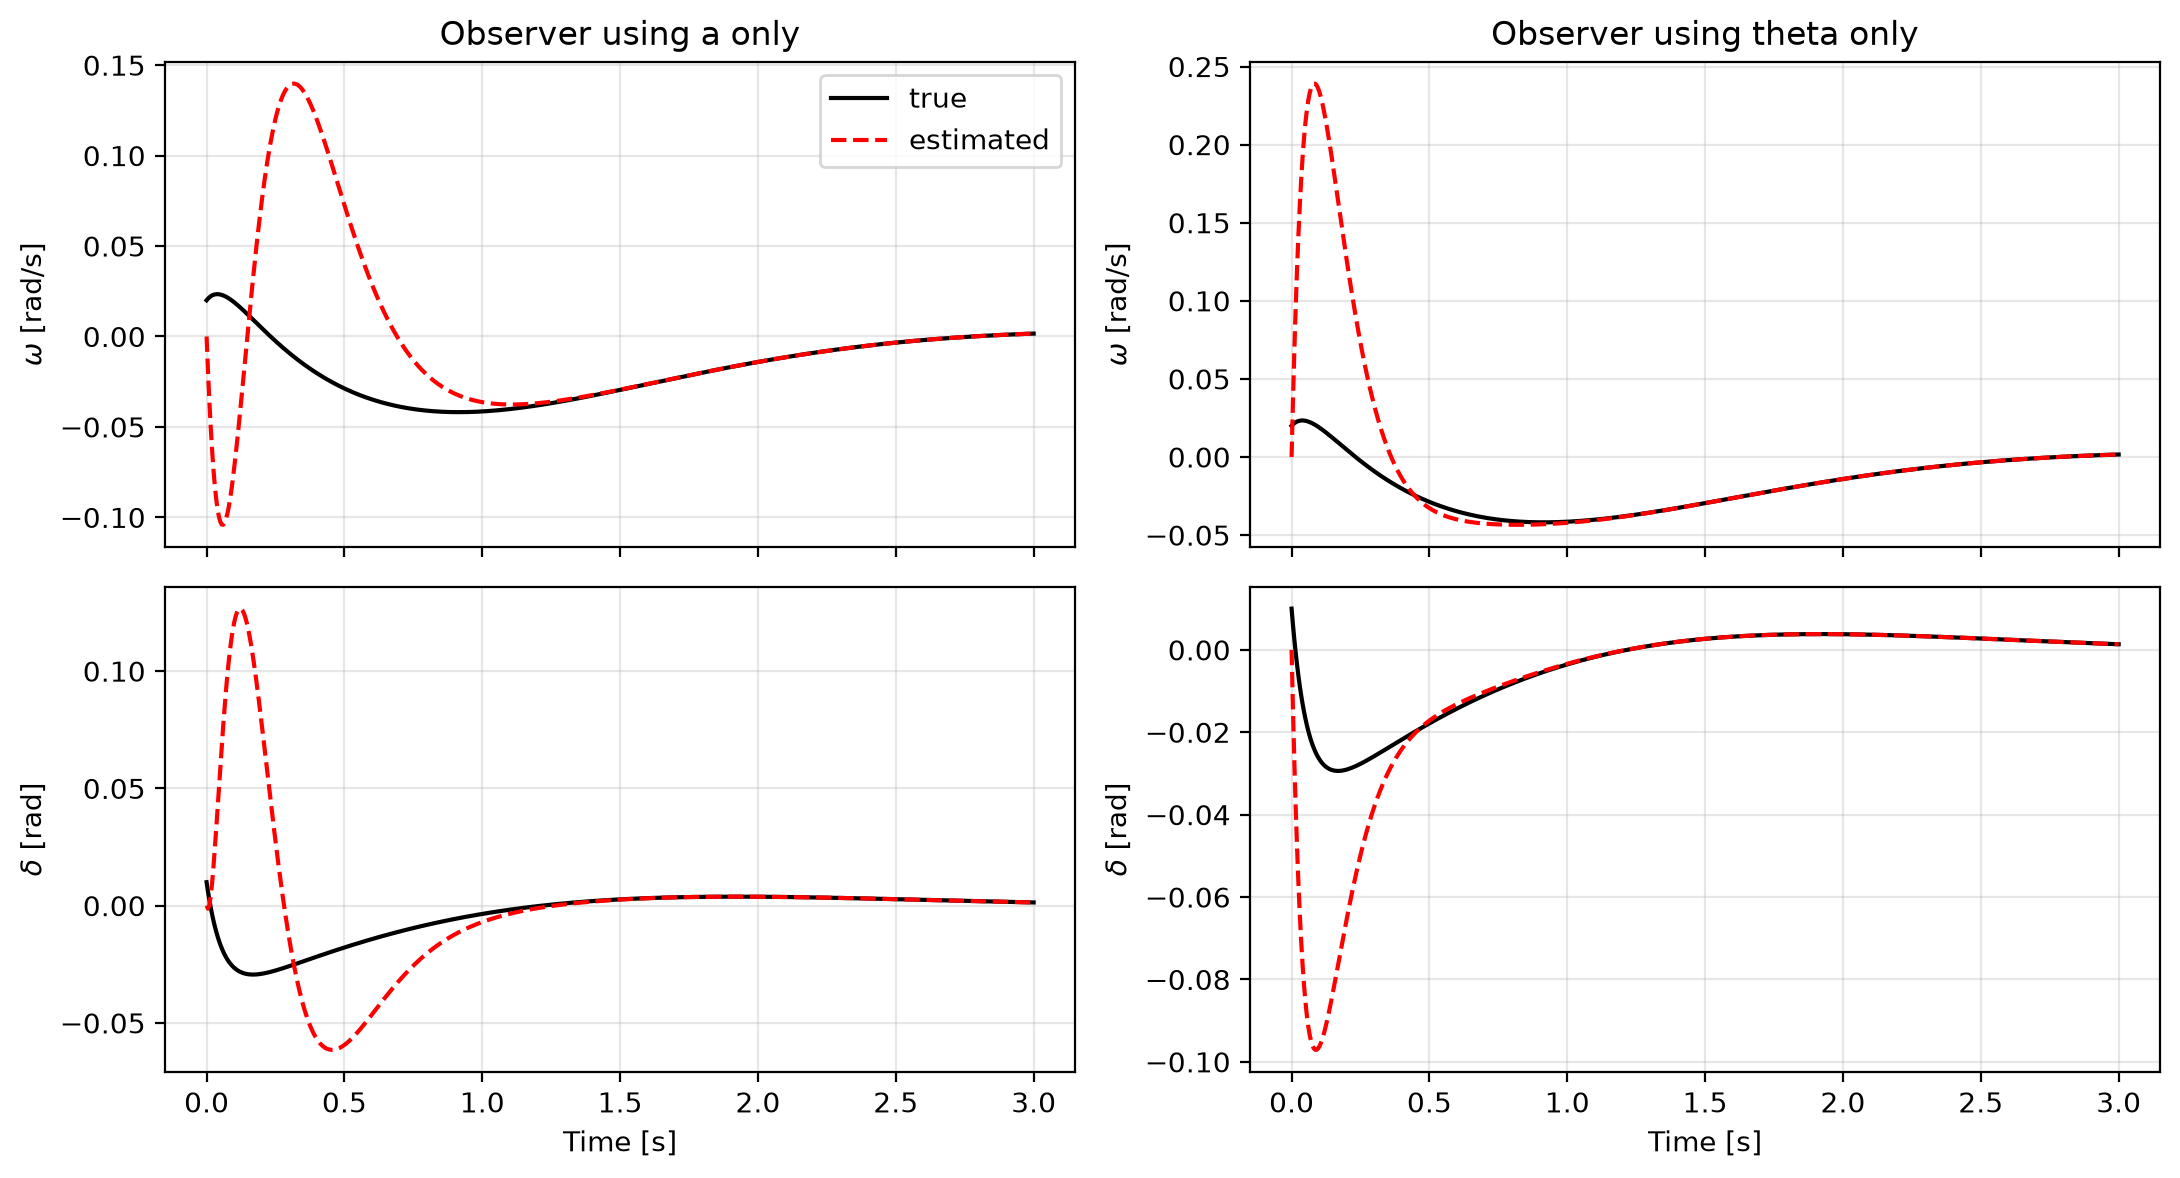
\includegraphics[width=0.85\textwidth]{fig_observer.png}
\caption{Estados reales (negro) y estimados por el observador (rojo discontinuo) con solo $a$ (izquierda) o solo $\theta$ (derecha).}\label{fig:obs}
\end{figure*}

Para comprobar que $\omega$ y $\delta$ se pueden reconstruir se dise\~n\'o un observador de Luenberger, un ``simulador del cohete'' que se corrige con las mediciones y que \emph{no conoce} el estado inicial (empieza en cero), al principio se equivoca y converge (figura~\ref{fig:obs}), con $a$ las curvas se superponen en 1 s y el error es de $\sim10^{-9}$ a los 3 s, con $\theta$ solo el pico inicial es mayor ($\omega$ estimada llega a 0,24 rad/s cuando la real es 0,02) y exige una ganancia de correcci\'on enorme ($|L|\approx3740$ frente a 22,5), la IMU es una ventana estrecha a $\omega$ y $\delta$, y reconstruirlos amplifica el ruido del sensor.

La pregunta inversa es la controlabilidad, ¿las \'ordenes pueden llevar al cohete a \emph{cualquier} estado?, se prob\'o con ambas entradas, con $u_1$ solo (falla del servo), con $u_2$ solo (falla del control de empuje), con el servo atascado ($\dot\delta=0$) y con $K_2=0$ (tabla~\ref{tab:ctrb}), con $u_1$ solo el rango es 4, el cohete es controlable en teor\'ia, pero con autoridad m\'inima ($\sigma_{\min}$ 907 veces menor), 10~\% de empuje inclina al cohete solo $1{,}03^\circ$, con el servo atascado o con $K_2=0$ el rango cae a 3, el estado $\delta$ queda fuera de alcance y el cohete adem\'as es inestable (polo $+0{,}557$), ninguna ley de control puede mover un estado no controlable, la tobera es la pieza cr\'itica y su p\'erdida es el peor escenario, el mismo de la inestabilidad con $K_2=0$, visto ahora como falta de alcance.

\begin{table}[!t]
\centering\small
\caption{Controlabilidad en distintos escenarios.}\label{tab:ctrb}
\begin{tabular}{lccc}
\toprule
Escenario & Rango & $\sigma_{\min}$ & Estable\\
\midrule
$u_1$ y $u_2$ (nominal) & 4 & 1,3 & s\'i\\
solo $u_1$ & 4 & 0,0014 & s\'i\\
solo $u_2$ & 4 & 1,3 & s\'i\\
servo atascado (solo $u_1$) & 3 & 0 & no\\
$K_2=0$ & 3 & 0 & no\\
\bottomrule
\end{tabular}
\end{table}


\subsection*{Selecci\'on de ganancias y periodo de muestreo}
Hasta aqu\'i casi todo par $(K_1,K_2)$ con $K_2\gtrsim0{,}09$ es estable, pero eso no basta, el nominal se pasa 16,4~\% y tarda 3,6 s, hay que elegir ganancias que den buen desempe\~no sin gastar de m\'as la tobera ni acoplar demasiado, se barri\'o una cuadr\'icula de 2400 pares ($K_1\in[0{,}5;20]$, $K_2\in[0{,}05;3]$) con cinco criterios sobre la respuesta a los escalones de $10$~\% y $5^\circ$ (los mismos del an\'alisis de acoplamiento), sobrepaso $M_p\le10$~\%, tiempo de asentamiento $t_s\le3$ s, error final $\le5$~\%, deflexi\'on m\'axima de tobera $\le5^\circ$ y $G_{11}(0)>0$; entre los puntos que cumplen todo se prefiere el de menor acoplamiento, medido como el peor de los dos porcentajes, los l\'imites son una elecci\'on de dise\~no del equipo; el l\'imite de tobera tambi\'en se refiere a esos escalones.

\begin{figure*}[!t]
\centering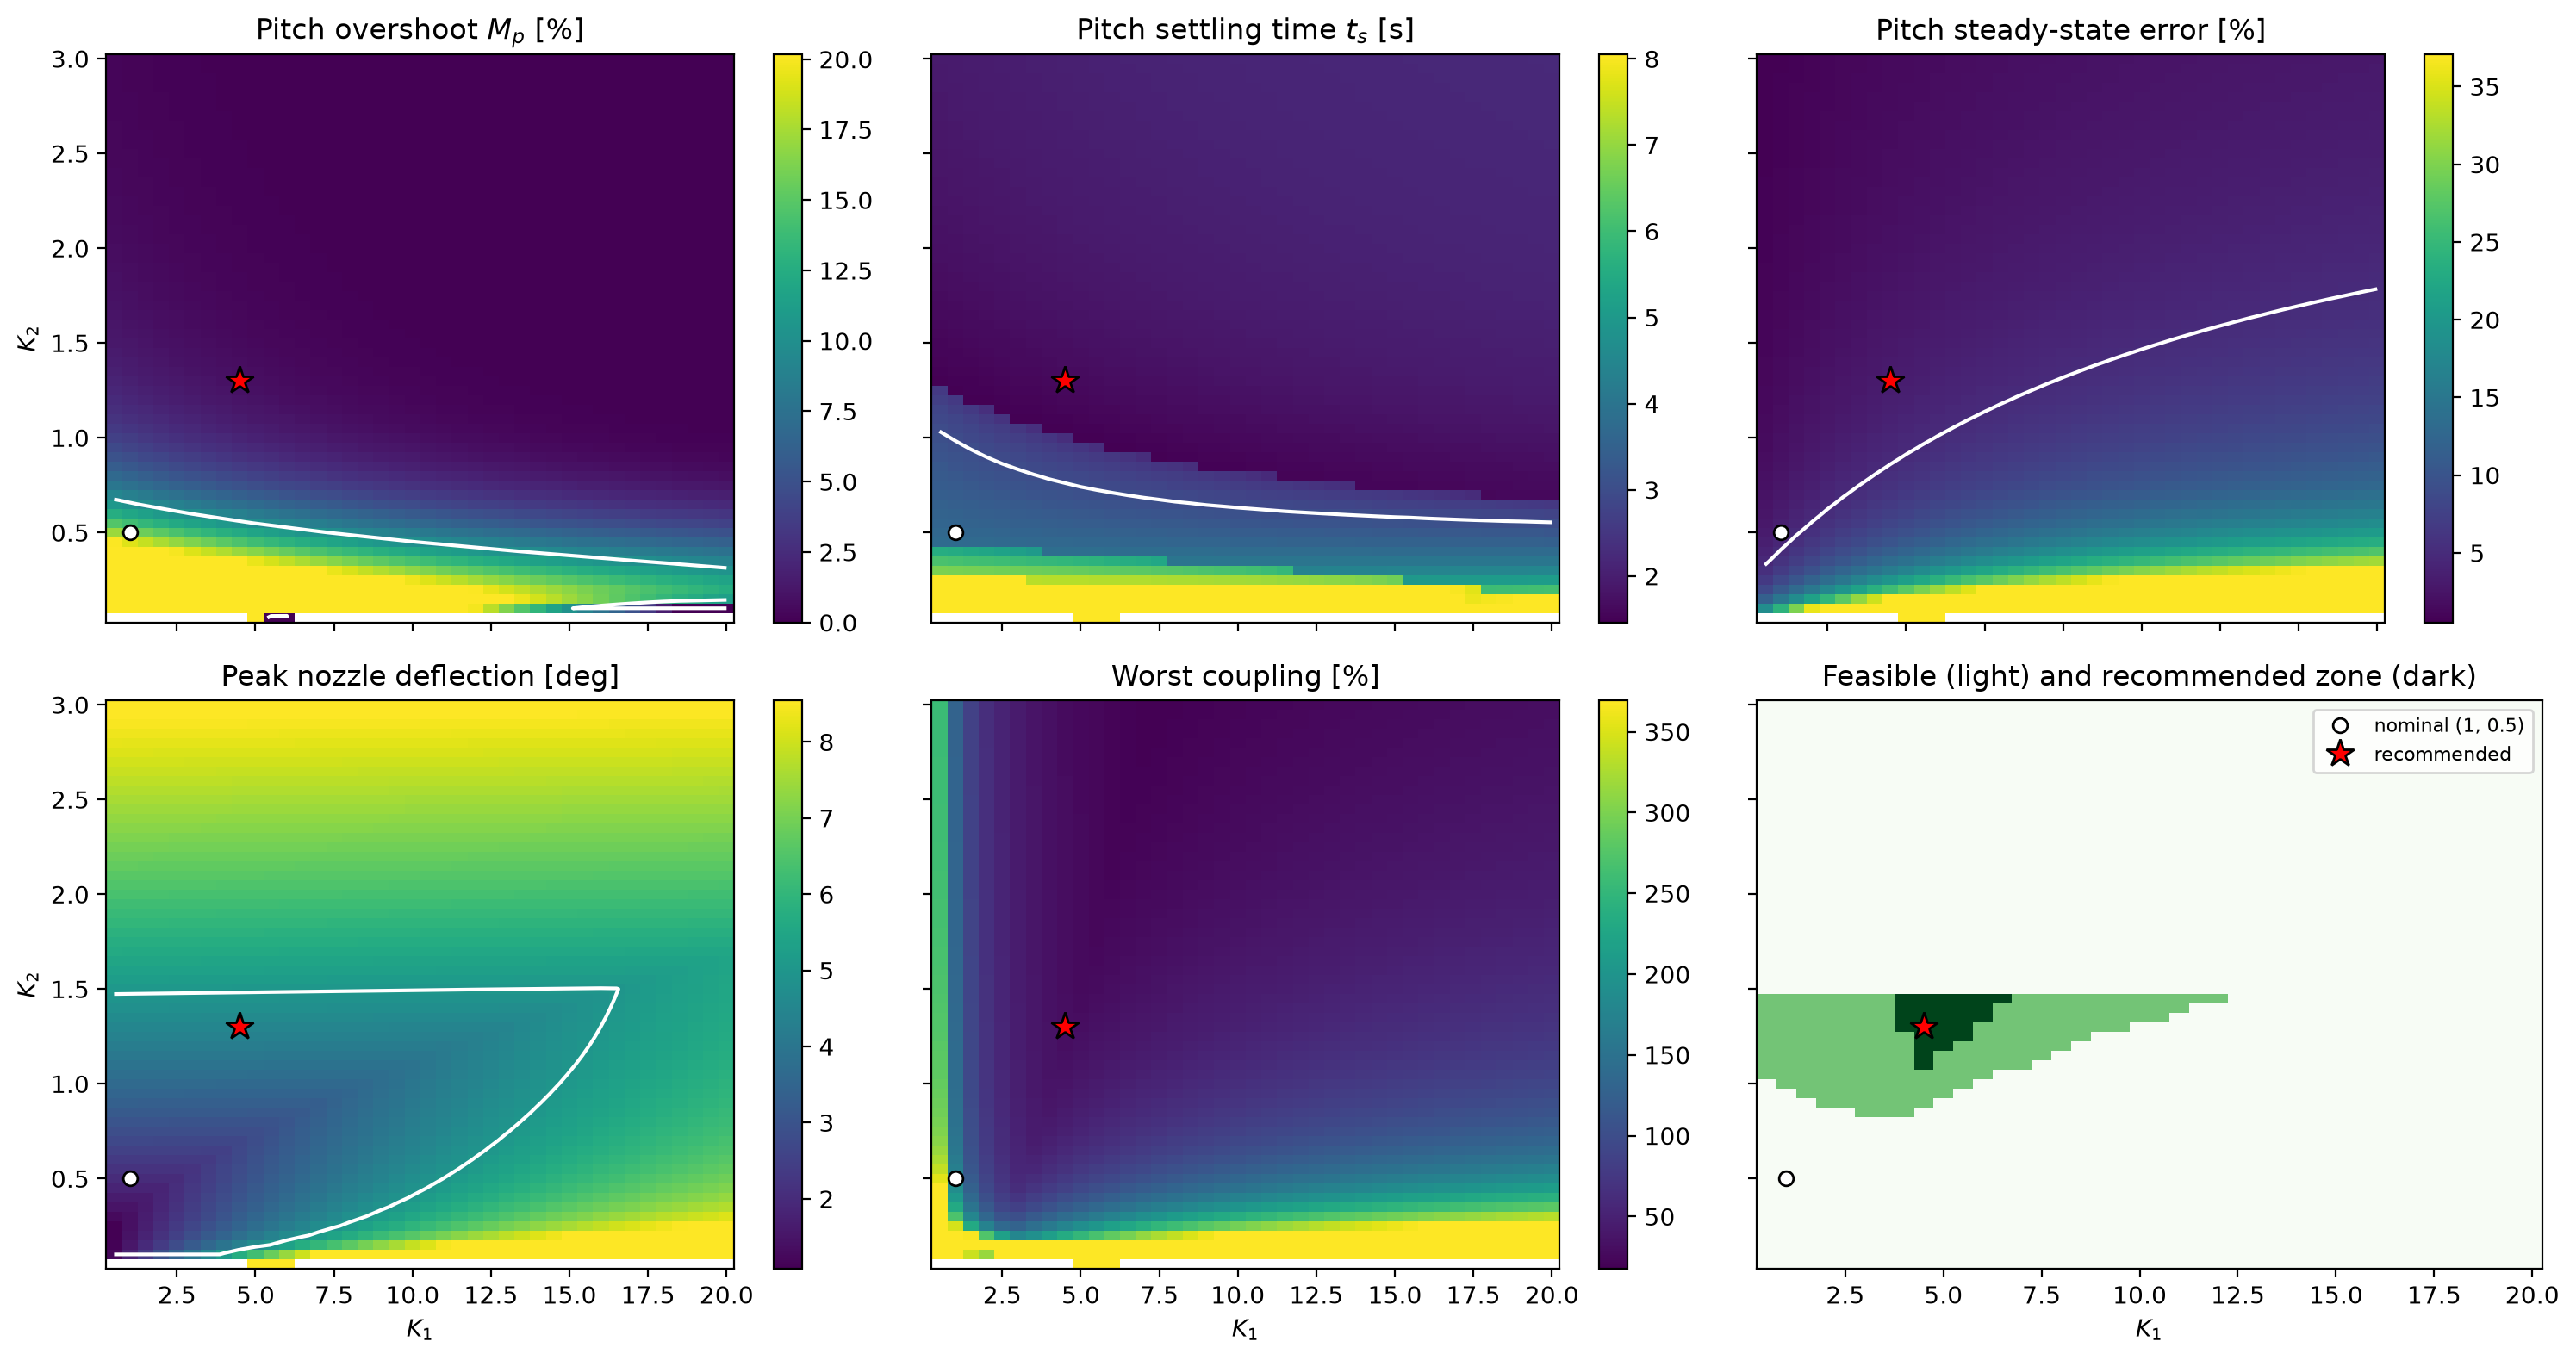
\includegraphics[width=0.9\textwidth]{fig_metric_maps.png}
\caption{Un mapa por criterio sobre el plano $(K_1,K_2)$; la l\'inea blanca es el l\'imite, $\circ$ es el nominal y $\star$ el recomendado, abajo a la derecha, zona factible (clara) y recomendada (oscura).}\label{fig:maps}
\end{figure*}

La figura~\ref{fig:maps} se lee as\'i, el color es el valor del criterio; oscuro es bajo y amarillo es alto, y como los cinco son ``costos'', oscuro es bueno, la escala se corta en el percentil 95 para que los pocos puntos casi inestables no aplasten los colores; la l\'inea blanca es el l\'imite y del lado oscuro se cumple.
\begin{itemize}
  \item \emph{Sobrepaso y tiempo} mejoran al subir $K_2$ (arriba, oscuro), con $K_2$ chico la tobera apenas contrarresta a $\mu$, los polos oscilatorios quedan poco amortiguados y el cohete cabecea de m\'as, el nominal queda debajo de la l\'inea (16,4~\% y 3,64 s).
  \item \emph{Error final}, la l\'inea sube con $K_1$, de $K_2\approx0{,}35$ a $\approx1{,}8$ para $K_1=20$, porque m\'as empuje inclina de m\'as al cohete por $k_\varepsilon$ ($G_{22}(0)=1{,}04$ con $K_1=1$ y $1{,}14$ con $K_1=10$) y hace falta m\'as $K_2$ para que la tobera mantenga el \'angulo pedido.
  \item \emph{Deflexi\'on de tobera}, es el \'unico criterio que encierra una regi\'on (solo 683 de 2400 puntos cumplen), arriba ($K_2\gtrsim1{,}5$) la tobera ordena demasiado por cada grado de error; a la derecha el mayor empuje la obliga a trabajar m\'as, fija el \emph{techo} $K_2\approx1{,}45$.
  \item \emph{Acoplamiento}, no tiene l\'imite, es lo que se minimiza; es m\'inimo hacia $K_1\gtrsim5$ con $K_2$ medio o alto.
\end{itemize}
La zona factible (187 puntos, $K_1\in[0{,}5;12]$, $K_2\in[0{,}85;1{,}45]$) es la intersecci\'on, el techo plano es la tobera y el borde inferior diagonal es el error final, que corta el techo hacia $K_1\approx12$, la zona recomendada, con acoplamiento a menos de 25~\% del mejor factible, es
\begin{gather}
K_1\in[4;\,6{,}5],\qquad K_2\in[1{,}1;\,1{,}45],\nonumber\\
(K_1,K_2)_{\text{rec}}=(4{,}5;\ 1{,}3).
\end{gather}
La tabla~\ref{tab:rec} compara el nominal con el punto recomendado, el sobrepaso baja casi a cero y el tiempo a menos de la mitad, y se reparte el acoplamiento (177~\% a 31~\% en $u_2\to a$) a costa de subir el otro de 21~\% a 28~\%; la tobera trabaja m\'as ($4{,}5^\circ$ de $5^\circ$ permitidos), los polos tambi\'en cambian, el modo lento pasa a $-1{,}6$ y aparece un par r\'apido y oscilatorio $-9{,}2\pm4{,}3j$ (el servo ahora se mezcla con el giro), es un compromiso, no un \'optimo \'unico.

\begin{table}[!t]
\centering\small
\caption{Nominal frente a recomendado.}\label{tab:rec}
\begin{tabular}{p{2.3cm}p{2.6cm}p{2.6cm}}
\toprule
 & Nominal $(1;0{,}5)$ & Recomendado $(4{,}5;1{,}3)$\\
\midrule
Sobrepaso $M_p$ de $\theta$ & 16,4~\% & 0,82~\%\\
Tiempo de asentamiento & 3,64 s & 1,62 s\\
Error final & 4,03~\% & 3,25~\%\\
Deflexi\'on de tobera m\'axima & $2{,}0^\circ$ & $4{,}5^\circ$\\
Acoplamiento $u_2\to a$ / $u_1\to\theta$ & 177~\% / 21~\% & 31~\% / 28~\%\\
Polos [s$^{-1}$] & $-17{,}3$; $-2{,}1$; $-1{,}07\pm1{,}2j$ & $-9{,}2\pm4{,}3j$; $-1{,}6\pm0{,}46j$\\
\bottomrule
\end{tabular}
\end{table}

En la realidad el controlador es una computadora, mide, calcula y ordena cada $T$ segundos y mantiene la orden constante entre muestras (retenedor de orden cero, la orden es una escalera), si $T$ es muy grande, el cohete cambi\'o demasiado entre correcciones y el lazo se vuelve inestable, como corregir el volante una vez por segundo; adem\'as el c\'omputo tarda, lo que se modela con un retardo de una muestra, se pregunta cu\'anto puede valer $T$ y si $T=0{,}05$ s es suficiente.

\begin{figure*}[!t]
\centering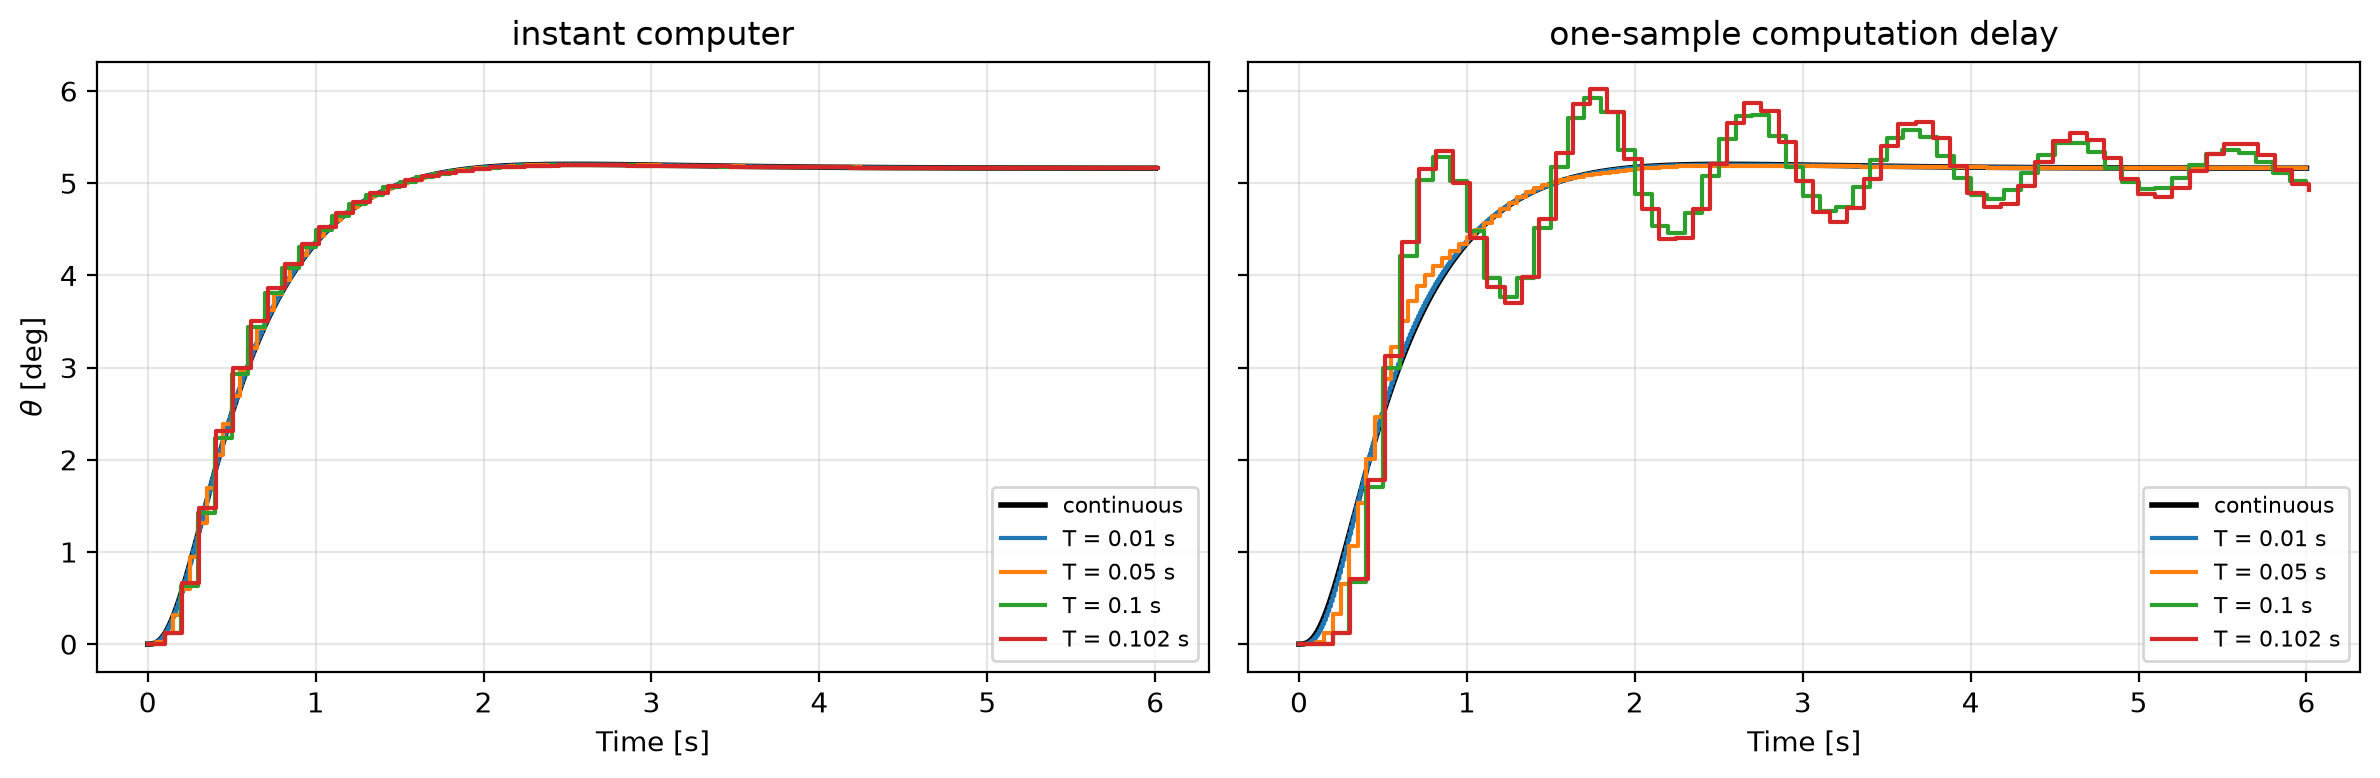
\includegraphics[width=0.85\textwidth]{fig_sampling.png}
\caption{Respuesta de $\theta$ a $u_2=5^\circ$ con las ganancias recomendadas, lazo continuo (negro) frente a muestreado (escalones), sin retardo (izquierda) y con retardo de una muestra (derecha).}\label{fig:sampling}
\end{figure*}

En la figura~\ref{fig:sampling}, con computadora instant\'anea, aun $T=0{,}1$ s casi coincide con la respuesta continua, con retardo, $T=0{,}05$ s sigue bien, pero con $T=0{,}1$ s la respuesta oscila alrededor de $5^\circ$ ($\pm1^\circ$) y no termina de asentarse, est\'a a punto de volverse inestable, un retardo hace que la correcci\'on llegue tarde, y en un cohete con un modo oscilatorio r\'apido como $-9{,}2\pm4{,}3j$ eso es peligroso, la regla pr\'actica pide entre 10 y 20 muestras dentro del tiempo de subida; con $T=0{,}05$ s hay 19 (subida de 0,97 s).

\begin{figure}[!t]
\centering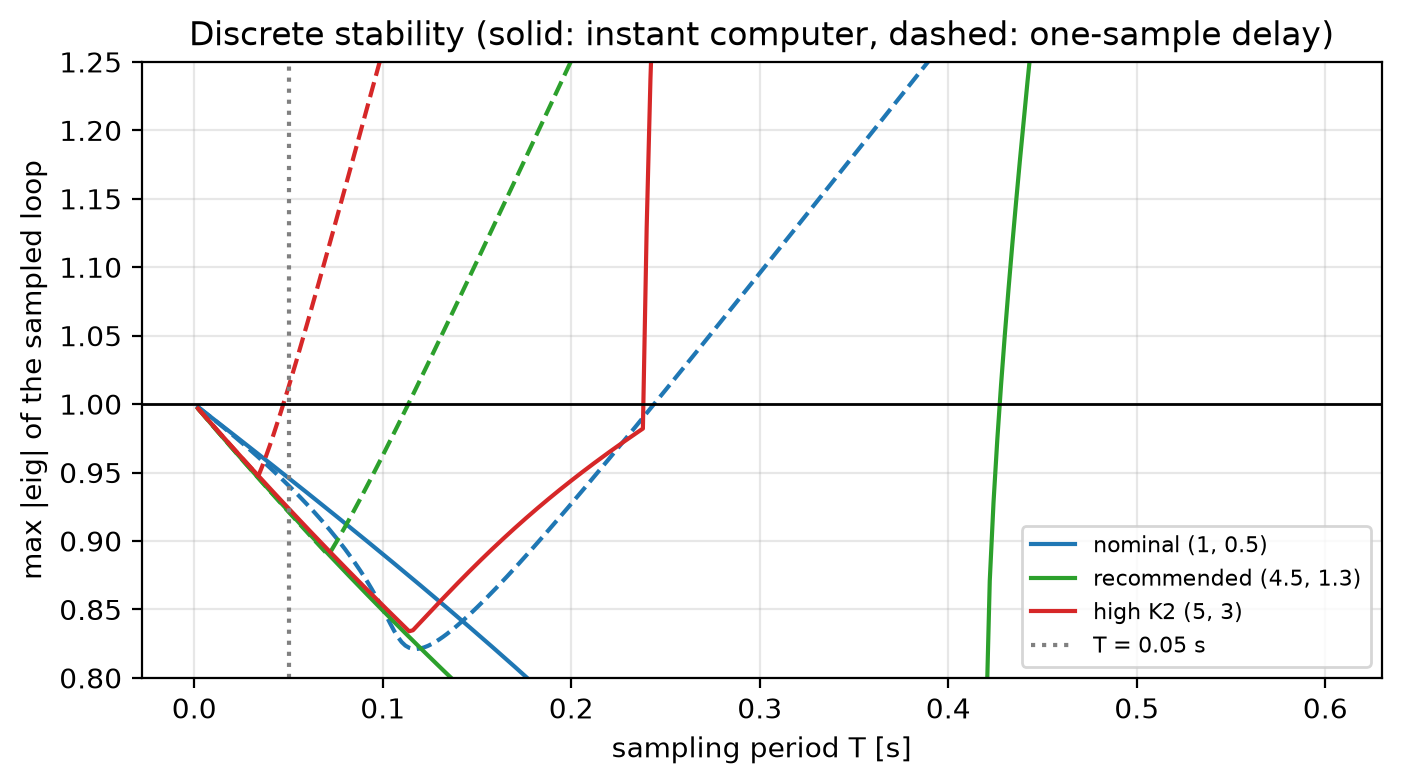
\includegraphics[width=\columnwidth]{fig_sampling_stability.png}
\caption{Radio espectral frente a $T$ (continua, sin retardo; discontinua, con retardo de una muestra).}\label{fig:rho}
\end{figure}

El radio espectral resume la estabilidad discreta en un solo n\'umero, mientras est\'e por debajo de 1 el lazo es estable (figura~\ref{fig:rho}), cada curva baja hasta un m\'inimo y despu\'es sube hasta cruzar 1, y ese cruce es el $T_{\max}$, la tabla~\ref{tab:tmax} muestra que con las ganancias recomendadas $T_{\max}$ en el peor caso (con retardo) es 0,114 s, es decir, $2{,}3$ veces el periodo elegido ($0{,}114/0{,}05$), la computadora podr\'ia ser 2,3 veces m\'as lenta antes de que el lazo se vuelva inestable, es un margen de seguridad, no una mejora de la respuesta, y es menor que el del nominal ($4{,}9\times$), subir $K_2$ mejora el sobrepaso y el tiempo de asentamiento, pero gasta margen de muestreo, con una $K_2$ alta, como $(5;3)$, el cociente es menor que uno y el lazo ser\'ia inestable con $T=0{,}05$ s.

\begin{table}[!t]
\centering\small\setlength{\tabcolsep}{3pt}
\caption{$T_{\max}$ y margen ($=T_{\max}$ con retardo$/0{,}05$ s).}\label{tab:tmax}
\begin{tabular}{lrrr}
\toprule
Ganancias & Sin retardo & Con retardo & Margen\\
\midrule
Nominal $(1;0{,}5)$ & 0,999 s & 0,244 s & $4{,}9\times$\\
Recomendado $(4{,}5;1{,}3)$ & 0,427 s & 0,114 s & $2{,}3\times$\\
Alta $K_2$ $(5;3)$ & 0,239 s & 0,047 s & $0{,}9\times$\\
\bottomrule
\end{tabular}
\end{table}

\begin{figure}[!t]
\centering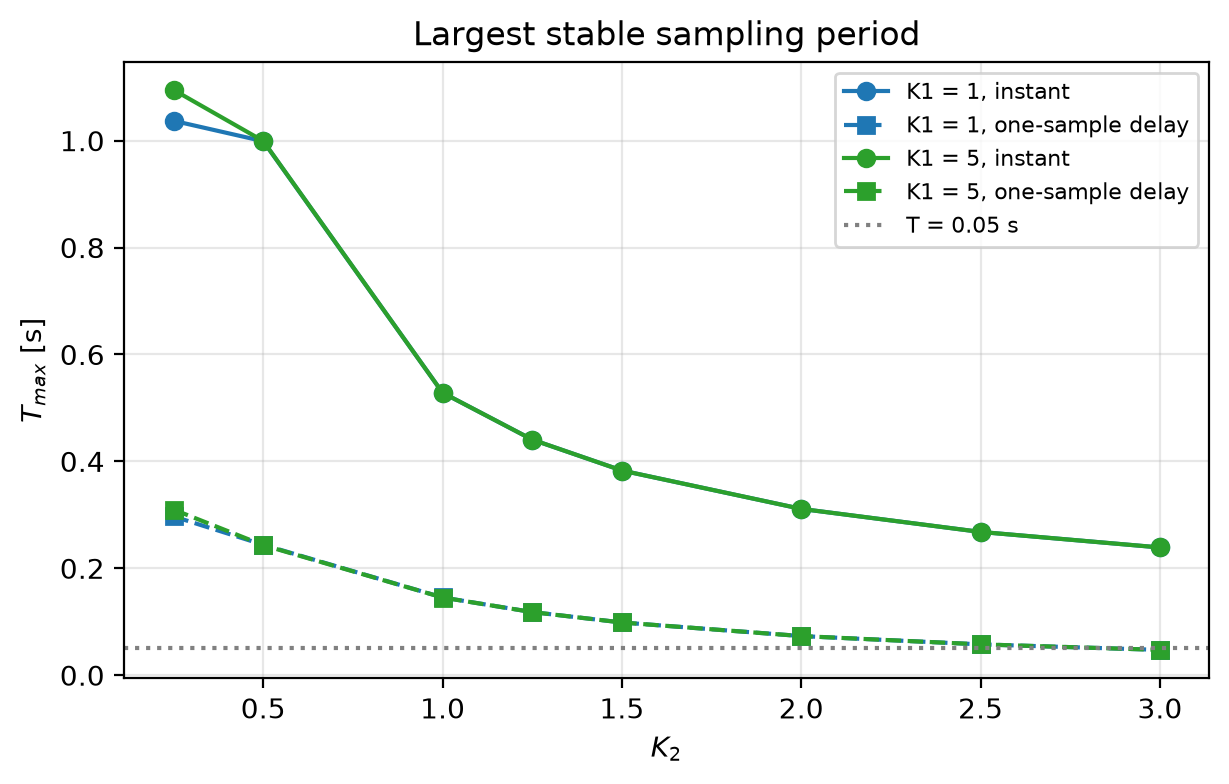
\includegraphics[width=\columnwidth]{fig_tmax_vs_k2.png}
\caption{$T_{\max}$ frente a $K_2$ para $K_1=1$ y $K_1=5$.}\label{fig:tmaxk2}
\end{figure}

La figura~\ref{fig:tmaxk2} muestra que $K_1$ casi no afecta a $T_{\max}$ (las curvas coinciden); lo que lo baja es $K_2$, de $\sim1$ s a $\sim0{,}24$ s sin retardo y de $\sim0{,}3$ a $\sim0{,}05$ s con retardo, $K_2$ gobierna el servo, el elemento r\'apido (polo $-17$), un servo con m\'as ganancia es m\'as ``nervioso'' y necesita corregirse con m\'as frecuencia, por eso no basta con subir $K_2$ todo lo posible, el techo de tobera es uno, y este es otro, de muestreo, el ancho de banda del cohete ($\sim2$ rad/s) es muy inferior a la frecuencia de muestreo ($2\pi/0{,}05\approx126$ rad/s), as\'i que el muestreo no es la limitaci\'on; lo es el retardo de c\'omputo combinado con ganancias altas de $K_2$.


\subsection*{Variaciones del modelo, masa variable y gui\~nada}
\textbf{Masa variable.} El motor quema combustible, con empuje constante $\dot m=-F_T/(I_{sp}g_0)$, y se supone la inercia proporcional a la masa, con $\rho(t)=m_0/m(t)\ge1$ ($\rho=2$ es un cohete a la mitad de su masa), los coeficientes que contienen $1/m$ o $1/I$ crecen con $\rho$, $k_a$, $k_\delta$, $\mu$ y $k_\varepsilon$ son proporcionales a $\rho$, mientras que $c_\theta$ y las constantes del motor y del servo no cambian, con inercia variable el balance de momentos es $I\dot\omega+\dot I\omega=M$, lo que a\~nade un t\'ermino que no existe en el modelo de coeficientes constantes, $\dot\omega=M/I-(\dot I/I)\,\omega$, como $\dot I/I=-\dot\rho/\rho$, el amortiguamiento pasa a ser $a_{d,\mathrm{eff}}=\rho\,a_{d0}-\dot\rho/\rho$ (un peque\~no anti-amortiguamiento), el modelo es el de las ecuaciones~(\ref{eq:a})--(\ref{eq:de}) con coeficientes que dependen del tiempo, $\dot x=A(t)x+B(t)u$, donde solo cambian $A_{11}$, $A_{31}$, $A_{32}$, $A_{33}$, $A_{34}$ y $B_{11}$, las ganancias $g_1$, $g_3$, $g_4$, $g_5$, $g_6$ y $g_7$ del diagrama (figura~\ref{fig:timevar}).

\begin{figure}[!t]
\centering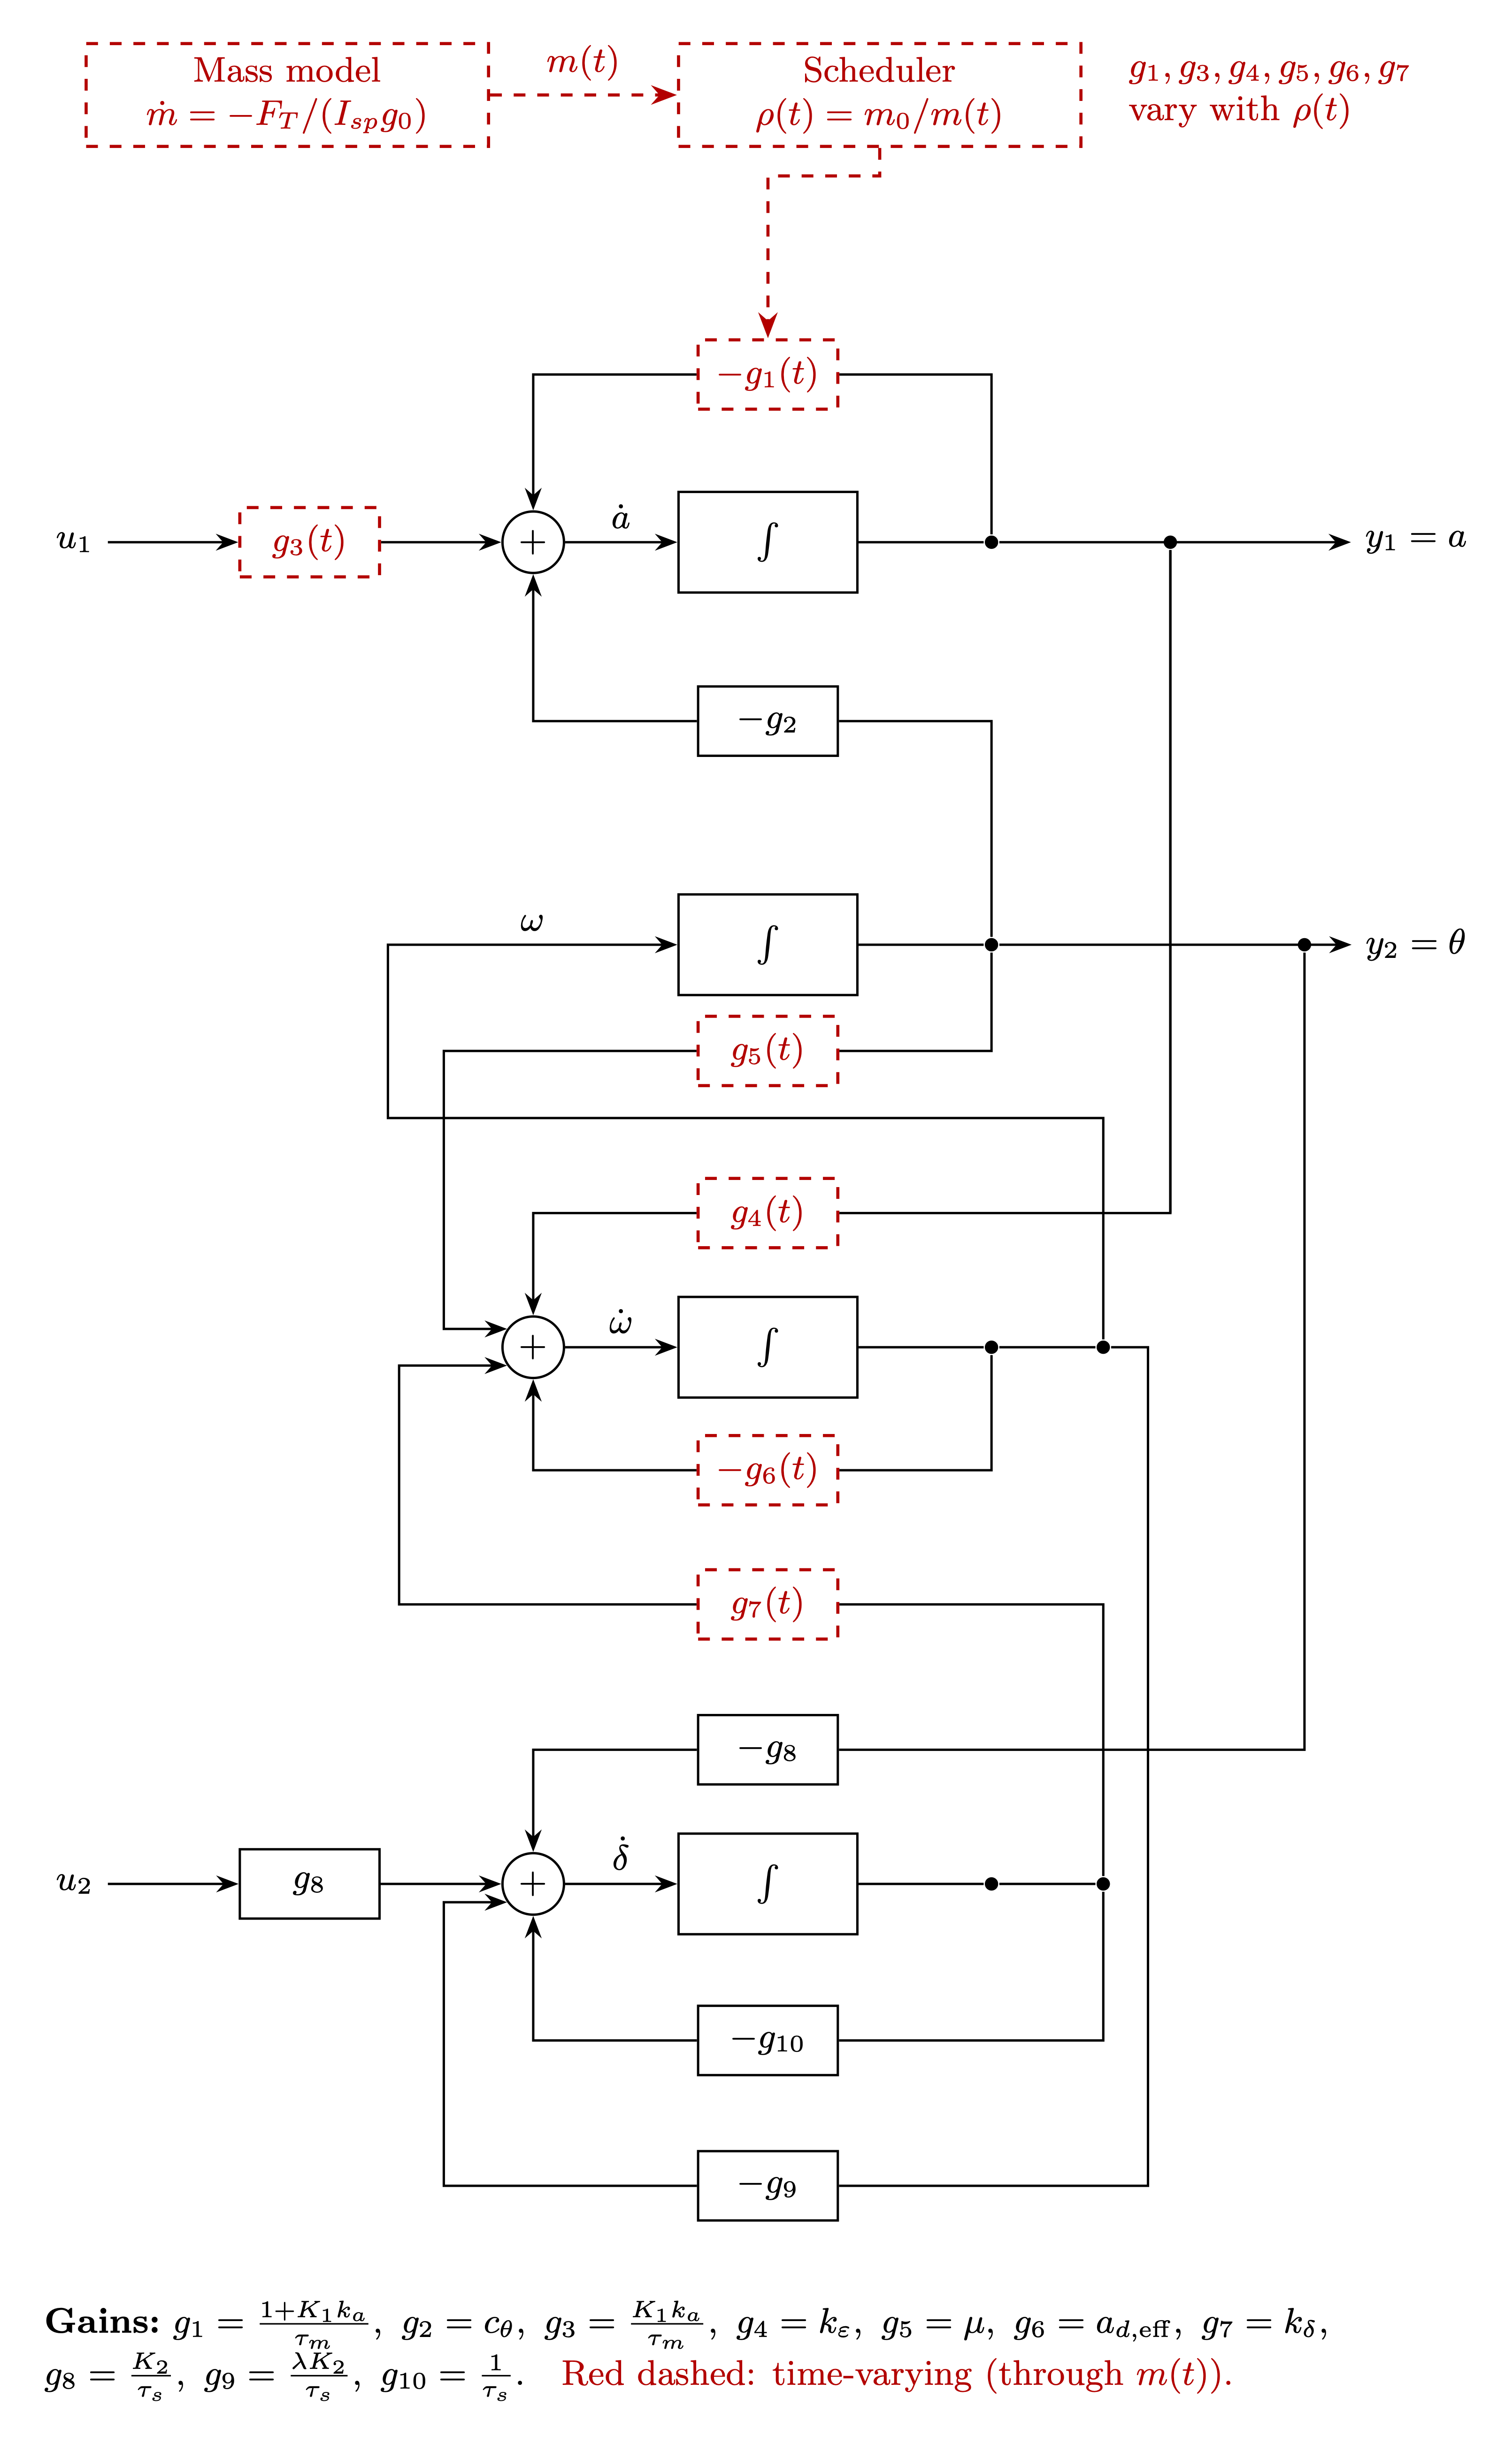
\includegraphics[width=\columnwidth]{fig_f15_timevar.png}
\caption{Diagrama con masa variable, en rojo, las ganancias que cambian con $m(t)$ a trav\'es de $\rho(t)$.}\label{fig:timevar}
\end{figure}

Con coeficientes que cambian ya no existen $G(p)$ ni polos fijos, porque ambos suponen coeficientes constantes; en su lugar se usa la matriz de transici\'on $\Phi(t,t_0)$, congelar $\rho$ en cada instante da un chequeo aproximado, v\'alido mientras la masa cambie despacio frente a la velocidad del lazo ($\sim1$ s), pero no demuestra estabilidad, como la ganancia del lazo crece con $\rho$, conviene \emph{programar las ganancias}, $K_1(t)=K_1/\rho$ y $K_2(t)=K_2/\rho$ dejan constantes $K_1k_a(t)$ y $k_\delta(t)K_2(t)$, en la figura~\ref{fig:frozen}, con ganancias fijas los polos lentos casi no se mueven ($\approx-1{,}6$), pero el par r\'apido se aleja del eje real, con parte imaginaria de $\pm4{,}3$ ($\rho=1$) a $\pm12{,}4$ ($\rho=2$), el cohete se vuelve m\'as ``vibrador'' porque la misma ganancia es ahora m\'as fuerte frente a la masa, sigue estable, pero $T_{\max}$ con retardo cae de 0,114 s a 0,058 s con $\rho=2$, casi igual al periodo elegido de 0,05 s, con ganancias programadas los polos casi no se mueven y $T_{\max}$ se mantiene entre 0,114 y 0,123 s, las ganancias recomendadas son v\'alidas al inicio del vuelo y conviene reajustarlas con la masa para conservar el margen de muestreo.

\begin{figure}[!t]
\centering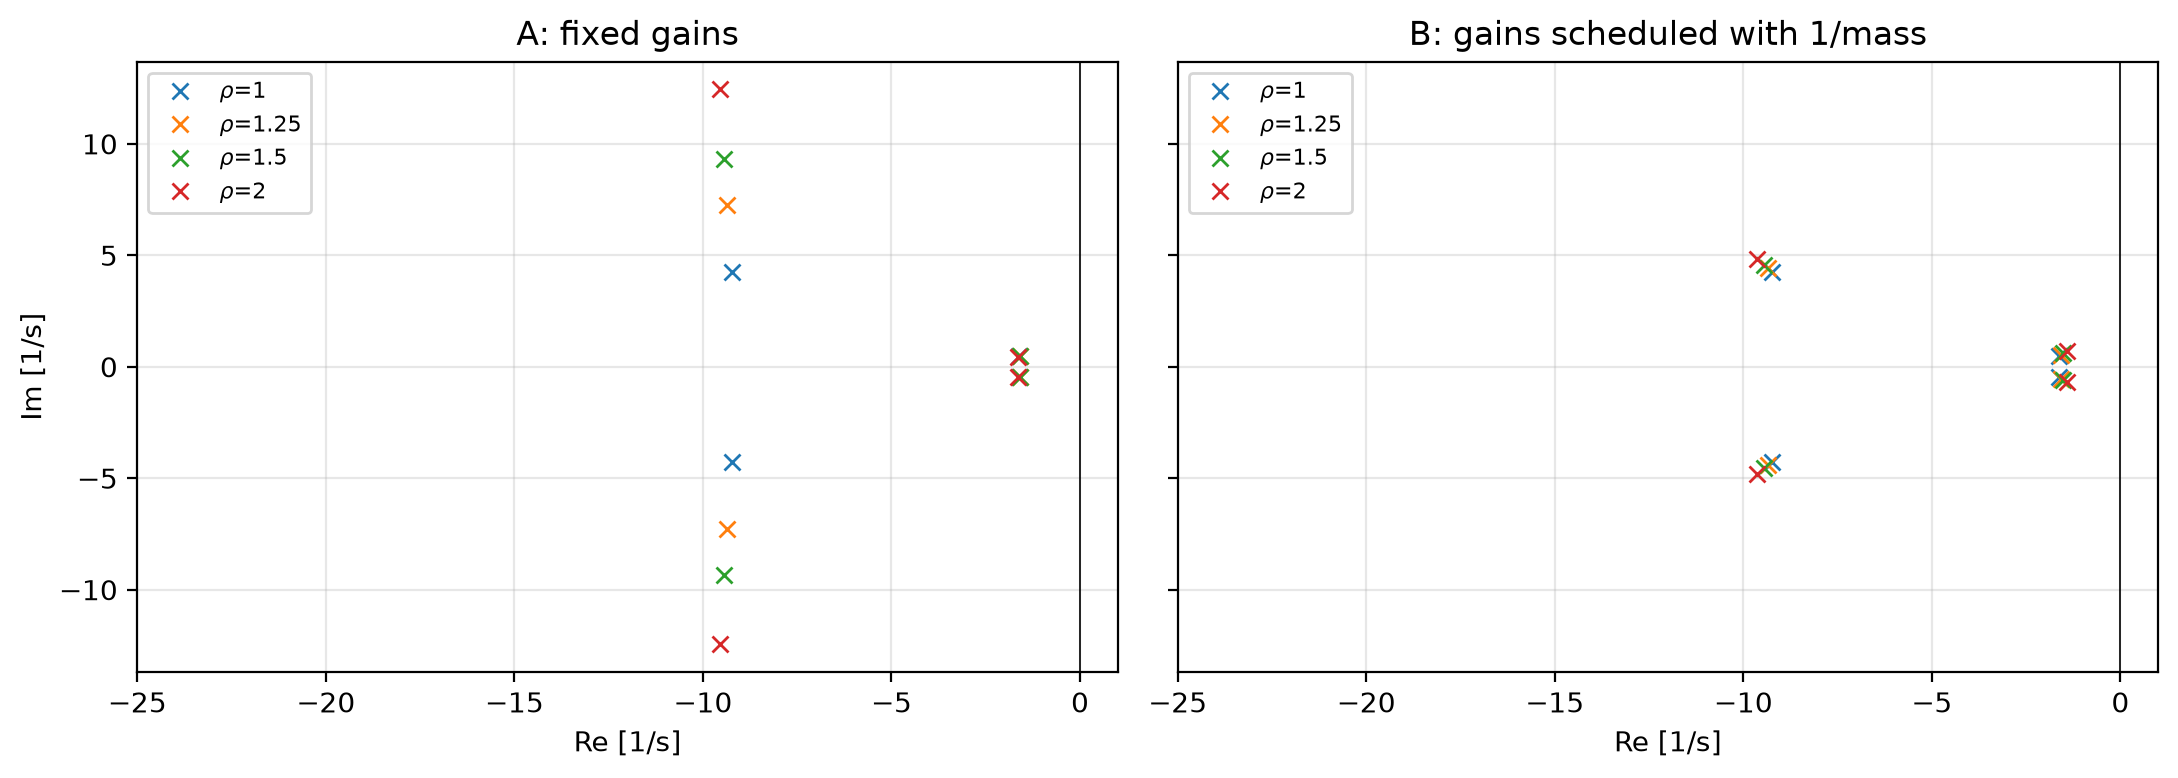
\includegraphics[width=\columnwidth]{fig_f15_frozen_poles.png}
\caption{Polos congelados al variar la masa, ganancias fijas (A) y programadas con $1/\rho$ (B).}\label{fig:frozen}
\end{figure}

\textbf{Gui\~nada como tercer canal.} Un cohete es casi sim\'etrico alrededor de su eje, as\'i que la gui\~nada (giro lateral) repite el cabeceo en el plano perpendicular, con su propia tobera, se a\~naden el \'angulo de gui\~nada $\psi$, su velocidad $r=\dot\psi$ y la deflexi\'on lateral $\zeta$, con un comando $u_3$ y una ganancia $K_3$ (\'angulos peque\~nos y sin alabeo):
\begin{align}
\dot\psi&=r,\qquad
\dot r=k_{\varepsilon\psi}\,a+\mu_\psi\,\psi-a_{d\psi}\,r+k_{\delta\psi}\,\zeta,\label{eq:yaw1}\\
\dot\zeta&=-\tfrac{1}{\tau_s}\,\zeta-\tfrac{K_3}{\tau_s}\,\psi-\tfrac{\lambda K_3}{\tau_s}\,r+\tfrac{K_3}{\tau_s}\,u_3,\label{eq:yaw2}
\end{align}
con $\mu_\psi=\mu$, $a_{d\psi}=a_d$, $k_{\delta\psi}=k_\delta$ y $k_{\varepsilon\psi}=k_\varepsilon$ (cohete sim\'etrico), con $x=[a,\theta,\omega,\delta,\psi,r,\zeta]^T$, $u=[u_1,u_2,u_3]^T$ y $y=[a,\theta,\psi]^T$ resultan 7 estados, 3 entradas y 3 salidas, con $A$ triangular por bloques, $A=\begin{bmatrix}A_{\text{cab}}&0\\K_{\psi a}&A_{\text{gui}}\end{bmatrix}$, donde $K_{\psi a}$ tiene una sola entrada distinta de cero, $k_{\varepsilon\psi}$ (de $a$ a $\dot r$), y $B_{\text{gui}}=[0\ 0\ K_3/\tau_s]^T$, ese es el \'unico enlace entre los dos planos (figura~\ref{fig:yaw}).

\begin{figure}[!t]
\centering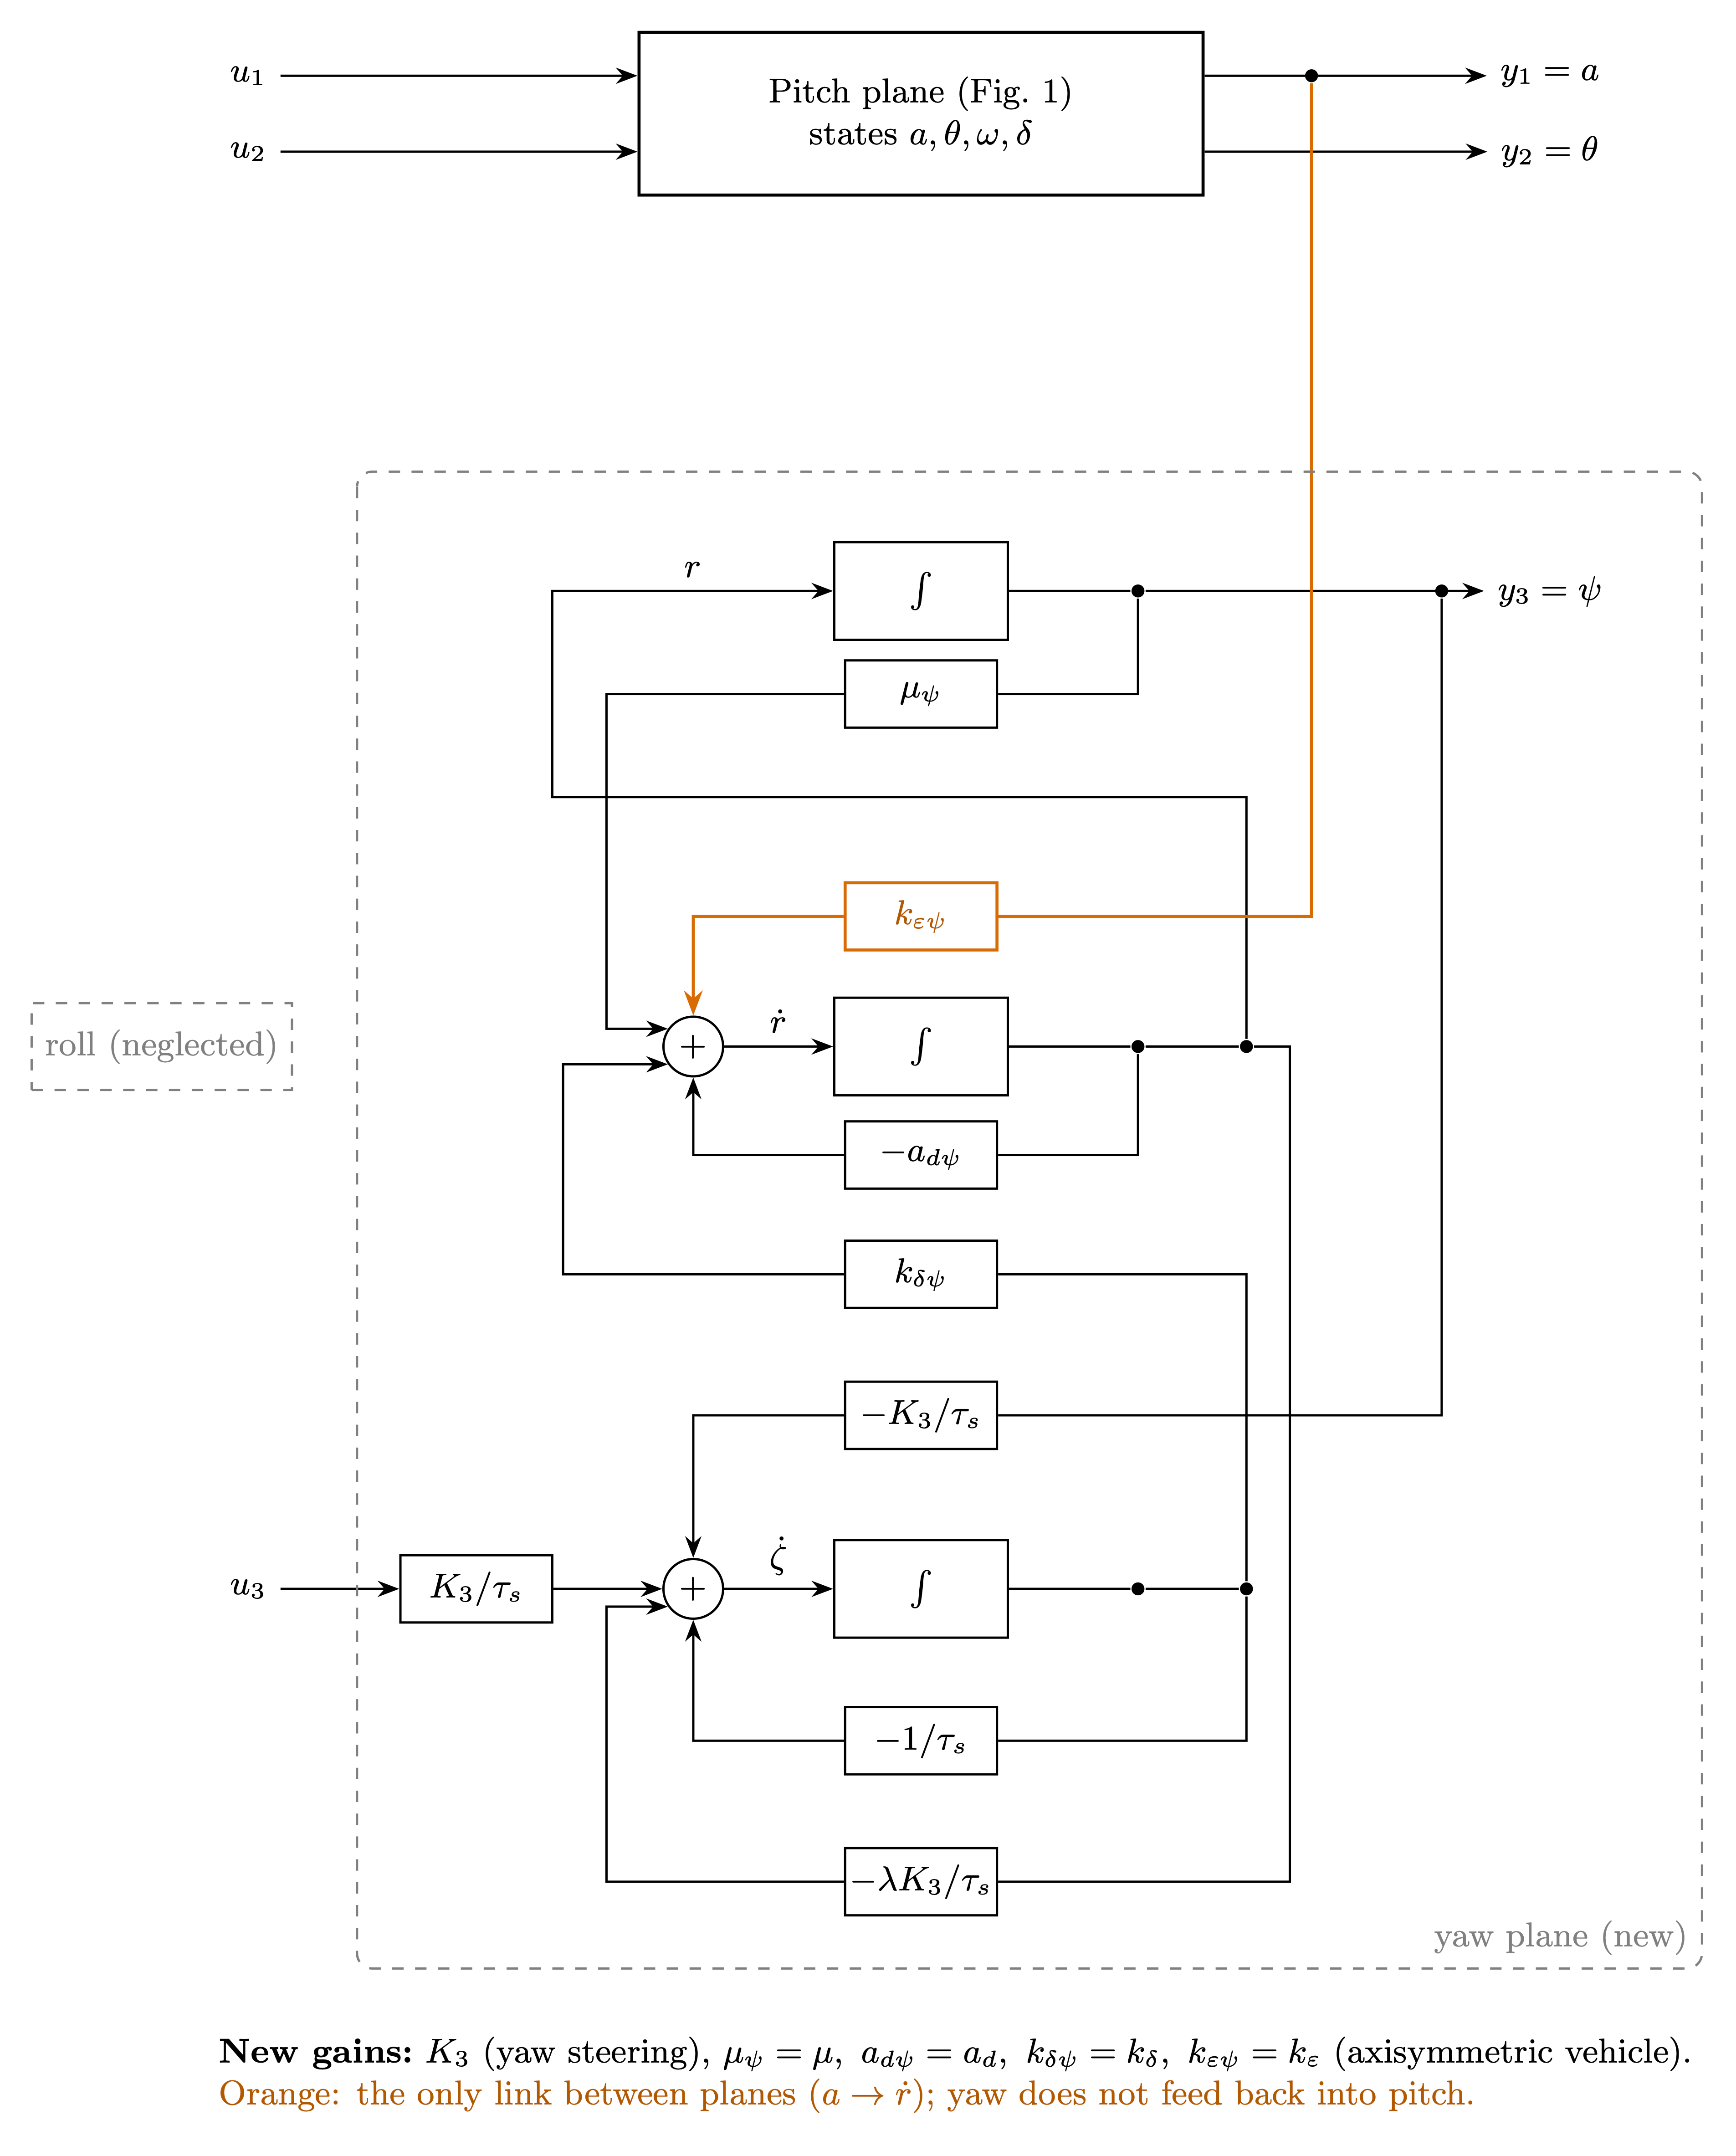
\includegraphics[width=\columnwidth]{fig_f15_yaw.png}
\caption{Diagrama con el canal de gui\~nada, el plano de cabeceo no cambia y el \'unico enlace entre planos es $a\to\dot r$.}\label{fig:yaw}
\end{figure}

Como $A$ es triangular por bloques, sus autovalores son los del cabeceo (los obtenidos para el plano de cabeceo) m\'as tres nuevos de la gui\~nada, de modo que la estabilidad se estudia por separado, la matriz de transferencia es $3\times3$ con ceros estructurales, $G_{13}=G_{23}=0$ ($u_3$ no mueve $a$ ni $\theta$) pero $G_{31}\ne0$ y $G_{32}\ne0$, pues la aceleraci\'on axial, que mueven tanto $u_1$ como $u_2$ (esta \'ultima por la gravedad), empuja la gui\~nada a trav\'es de $k_{\varepsilon\psi}$, el acoplamiento es entonces en un solo sentido, el cabeceo y el empuje perturban la gui\~nada, pero no al rev\'es; subir $K_1$ aumenta el acoplamiento $u_1\to\psi$, como $u_1\to\theta$ en el cabeceo, esto pasa de dos a tres canales, pero no es todav\'ia un modelo tridimensional completo, falta el alabeo, que en un cohete real acopla cabeceo y gui\~nada en ambos sentidos, y tampoco hay posici\'on lateral, solo orientaci\'on.


%====================================================================
\section{Discusi\'on}
\textbf{La inestabilidad es el punto de partida y la tobera la resuelve.} Por $\mu>0$ el aire tiende a voltear al cohete, y solo el servo, gobernado por $K_2$, lo evita, sin $K_2$ hay un polo en $+0{,}557$ s$^{-1}$ y con el servo atascado se pierde incluso la controlabilidad de $\delta$, basta $K_2\gtrsim0{,}09$ para estabilizar, y el mapa de estabilidad casi no depende de $K_1$, que pertenece a un canal que ya era estable, esto confirma la primera parte de la hip\'otesis.

\textbf{Dos sistemas independientes o un solo sistema MIMO.} La gravedad domina el acoplamiento, inclinar el cohete le resta m\'as aceleraci\'on (177~\%) de la que le da el empuje, mientras que el efecto inverso, por la desalineaci\'on, es mucho menor (21~\%), tratar al cohete como dos sistemas independientes solo es razonable para maniobras r\'apidas, por encima de unos 5 rad/s, donde ambos acoplamientos caen bajo 10~\%; para comandos que var\'ian despacio se subestimar\'ia el efecto de la inclinaci\'on sobre la aceleraci\'on, el mismo acoplamiento que estorba es el que permite \emph{ver} los estados no medidos, sin \'el, el cohete ser\'ia opaco para los sensores.

\textbf{El efecto de $K_1$ y $K_2$.} Cada ganancia tiene su trabajo, $K_2$ gobierna la actitud (amortiguamiento, rapidez del giro) y la estabilidad, pero un valor alto gasta tobera y baja el periodo de muestreo permitido; $K_1$ gobierna cu\'anta aceleraci\'on se logra con un comando de empuje y reduce el acoplamiento gravitacional, pero aumenta el acoplamiento inverso, de ah\'i que existan una zona factible y una zona recomendada acotadas por la tobera (techo de $K_2$), por el error final y por el acoplamiento; el resultado es un compromiso.

\textbf{El efecto del muestreo.} El ancho de banda del cohete ($\sim2$ rad/s) es muy inferior a la frecuencia de muestreo, as\'i que $T=0{,}05$ s es suficiente con las ganancias recomendadas; la limitaci\'on es el retardo de c\'omputo combinado con $K_2$ alto, y empeora si la masa disminuye durante el vuelo, lo que justifica programar las ganancias.

\textbf{L\'imites del modelo.} Todo se obtuvo con un modelo lineal de \'angulos peque\~nos, par\'ametros constantes, fuselaje r\'igido y escalones elegidos por el equipo; la recomendaci\'on de ganancias vale para esos escalones y para el l\'imite de tobera adoptado, y con otras magnitudes el punto recomendado se desplaza, no se modelaron saturaciones del motor y de la tobera, flexibilidad estructural, oleaje del propelente ni el alabeo.

%====================================================================
\section{Conclusi\'on}
Se estudi\'o un modelo lineal MIMO del cohete en el plano de cabeceo, el cohete es inestable por naturaleza y la tobera lo estabiliza con $K_2\gtrsim0{,}09$, con las ganancias de partida $(1;0{,}5)$ el cohete es estable pero el acoplamiento por gravedad es severo (177~\%) y la respuesta es lenta y oscilante, el rango recomendado, $K_1\in[4;6{,}5]$ y $K_2\in[1{,}1;1{,}45]$, con punto $(4{,}5;1{,}3)$, da sobrepaso de 0,8~\%, tiempo de asentamiento de 1,6 s y acoplamientos de 31~\% y 28~\%, a costa de usar casi toda la tobera, con dos sensores se pueden reconstruir los estados no medidos, aunque medir solo $\theta$ es fr\'agil; sin tobera no hay control posible, un periodo de muestreo de 0,05 s es suficiente, el periodo m\'aximo estable (0,114 s) es $2{,}3$ veces mayor, incluso con retardo de c\'omputo, con masa variable las ganancias deber\'ian programarse con $1/\rho$, y la gui\~nada se a\~nade como un segundo plano acoplado en un solo sentido, aprendimos que el comportamiento de un sistema multivariable se entiende mejor siguiendo la cadena f\'isica causa--efecto que mirando cada canal por separado.

%====================================================================
\begin{thebibliography}{9}

\bibitem{nasa}
NASA Glenn Research Center, \emph{Rocket Control. Beginner's Guide to Aeronautics}, \url{https://www1.grc.nasa.gov/beginners-guide-to-aeronautics/rocket-control/}.

\bibitem{nise}
N.~S. Nise, \emph{Control Systems Engineering}, 7th ed., John Wiley \& Sons, 2019.

\bibitem{ogata}
K.~Ogata, \emph{Modern Control Engineering}, 5th ed., Prentice Hall, 2010.

\bibitem{franklin}
G.~F. Franklin, J.~D. Powell and M.~Workman, \emph{Digital Control of Dynamic Systems}, 3rd ed., Addison-Wesley, 1998.

\bibitem{skogestad}
S.~Skogestad and I.~Postlethwaite, \emph{Multivariable Feedback Control: Analysis and Design}, 2nd ed., John Wiley \& Sons, 2005.

\bibitem{wie}
B.~Wie, \emph{Space Vehicle Dynamics and Control}, 2nd ed., AIAA Education Series, 2008.

\bibitem{greensite}
A.~L. Greensite, \emph{Analysis and Design of Space Vehicle Flight Control Systems}, Spartan Books, 1970.

\end{thebibliography}

\end{document}
